\chapter{Assembly}


\section{Funzioni}
Per definire una funzione utilizziamo una "etichetta"/"label".
Una funzione si definisce nel seguente modo $\rightarrow$ nome\_etichetta 
\\esempio funzione somma:

\begin{verbatim}
    SOMMA:
\end{verbatim}

\noindent Per rendere una funzione visibile da altri file oggetto usiamo la direttiva ".globl". esempio

\begin{verbatim}
    .globl SOMMA
    SOMMA:
\end{verbatim}

\noindent esempio prima parte, codice C $\rightarrow$ Assembly\medskip\\
\begin{minipage}{0.4\textwidth}
\begin{verbatim}
int f(){
    int x;
    x = 10;
    return x;
}
\end{verbatim}
\end{minipage}
\hfill
$\longrightarrow$
\hfill
\begin{minipage}{0.4\textwidth}
\begin{verbatim}
.globl f
f:
#x -> eax //prende tutto il registro
\end{verbatim}
\end{minipage}
\noindent

\subsection{Uso di parametri nelle funzioni}
\begin{minipage}{0.3\textwidth}
\begin{verbatim}
 int f(int x){
        return x+1;
    }


    
f.c
\end{verbatim}
\end{minipage}
\hfill
$\longrightarrow$
\hfill
\begin{minipage}{0.3\textwidth}
\begin{verbatim}
int f(int x){
    int a;
    a=x;
    a++;
    return a;
}

f_eq.c
\end{verbatim}
\end{minipage}
\hfill
$\longrightarrow$
\hfill
\begin{minipage}{0.3\textwidth}
\begin{verbatim}
.globl f
f:
#a->eax
movl ,%eax
inc %eax
ret

f.s
\end{verbatim}

\end{minipage}
\noindent
\section{Istruzioni}
Per ogni istruzione dobbiamo definire la taglia dei dati su cui andrà a operare seguendo la sua semantica. In IA32 abbiamo tre tagli possibili:

\begin{table}[H]
    \centering
    \begin{tabular}{|c|c|c|}
    \hline
         Esempio & Suffisso Assembly & Dimensione in byte\\
         \hline
         Char & b & 1 \\
         Short & w & 2 \\
         int, T* & l & 4 \\
         \hline
    \end{tabular}
\end{table}
\noindent



\subsubsection{Istruzioni per lo spostamento}
S viene spostato in D

\begin{verbatim}
    mov  S, D
\end{verbatim}

\noindent le istruzioni hanno in generale un operando sorgente che specifica un valore di ingresso per l'operazione e un operando destinazione che identifica dove deve essere immagazzinato il risultato

\begin{itemize}[label=--]
    \item Operando Sorgente
    \begin{itemize}
    \item Immediato $\rightarrow$ operando immagazzinato insieme all'istruzione stessa dichiarato con \$, esempio \$10
    \item Registro $\rightarrow$ operando memorizzato in  uno degli 8 registri interni dichiarato con \%, esempio \%eax
    \item Memoria $\rightarrow$ opera memorizzato in memoria
    \end{itemize}
    \item Operando Destinazione
    \begin{itemize}
        \item Registro $\rightarrow$ il risultato dell'operazione viene memorizzato in uno degli 8 registri interni, sempre dichiarato con \%
        \item Memoria $\rightarrow$ il risultato dell'operazione viene memorizzato in memoria
    \end{itemize}
\end{itemize}

\noindent \textcolor{red}{\textbf{Regola}:}
non si usano mai valori immediati per l'operando D
\\ \textcolor{red}{\textbf{Regola}:} non è possibile usare l'indirizzamento a memoria per entrambi gli operandi
\medskip\\esempio seconda parte, codice C $\rightarrow$ Assembly\medskip\\
\begin{minipage}{0.4\textwidth}
\begin{verbatim}
int f(){
    int x; // dichiarazione
    x = 10; // assegnazione
    return x;
}

f.c
\end{verbatim}
\end{minipage}
\hfill
$\longrightarrow$
\hfill
\begin{minipage}{0.4\textwidth}
\begin{verbatim}
.globl f
f:
#x -> eax //prende tutto il registro
movl $10, %eax
ret

f.s
\end{verbatim}
\end{minipage}
\bigskip\\esempio con char codice C $\rightarrow$ Assembly\medskip\\
\begin{minipage}{0.4\textwidth}
\begin{verbatim}
char f(){
    char p; // dichiarazione
    p = 'a'; // assegnazione
    printf(%"c\n",p)
    return 0;
}

f.c
\end{verbatim}
\end{minipage}
\hfill
$\longrightarrow$
\hfill
\begin{minipage}{0.4\textwidth}
\begin{verbatim}
.globl f
f:
#x -> al //prende tutto il registro
movb $0x61, %al
ret

f.s
\end{verbatim}
\end{minipage}
\subsection{Struttura dei dati in memoria}
Per la struttura dei dati in memoria vediamo nello specifico il funzionamento dello StackPointer:
\begin{figure}[H]
    \centering
    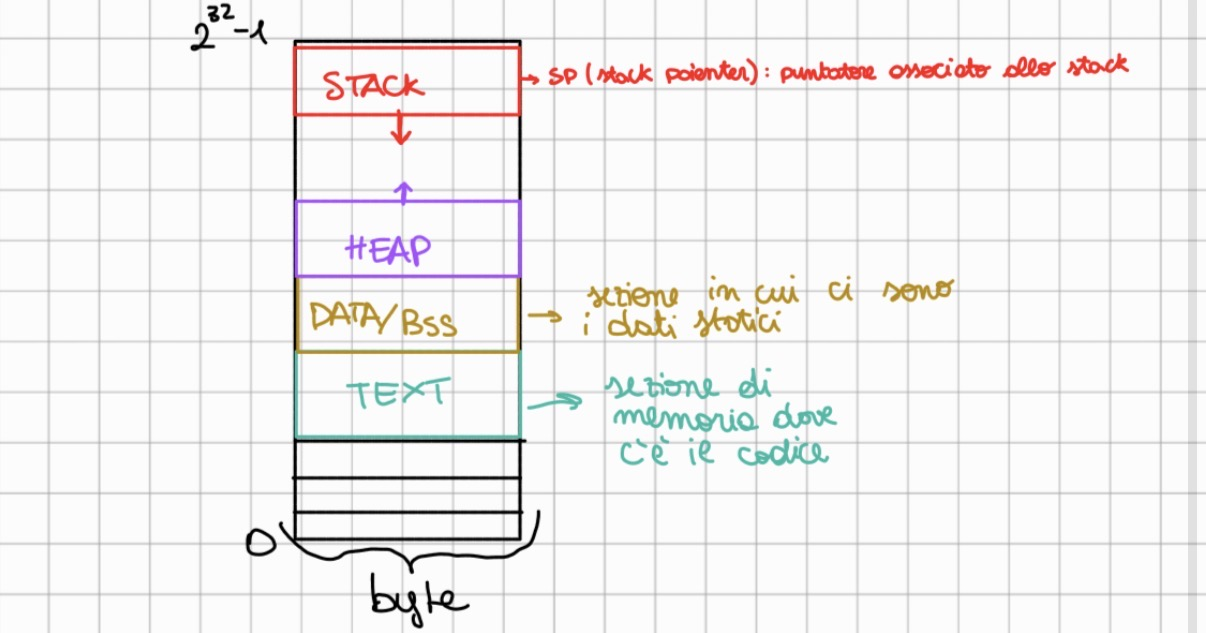
\includegraphics[width=0.7\linewidth]{../images/StackPointer1.jpg}
    \caption{StackPointer}
\end{figure}
Vediamo però cosa accade di preciso nella memoria quando viene chiamata la funzione f:
\begin{figure}[H]
    \centering
    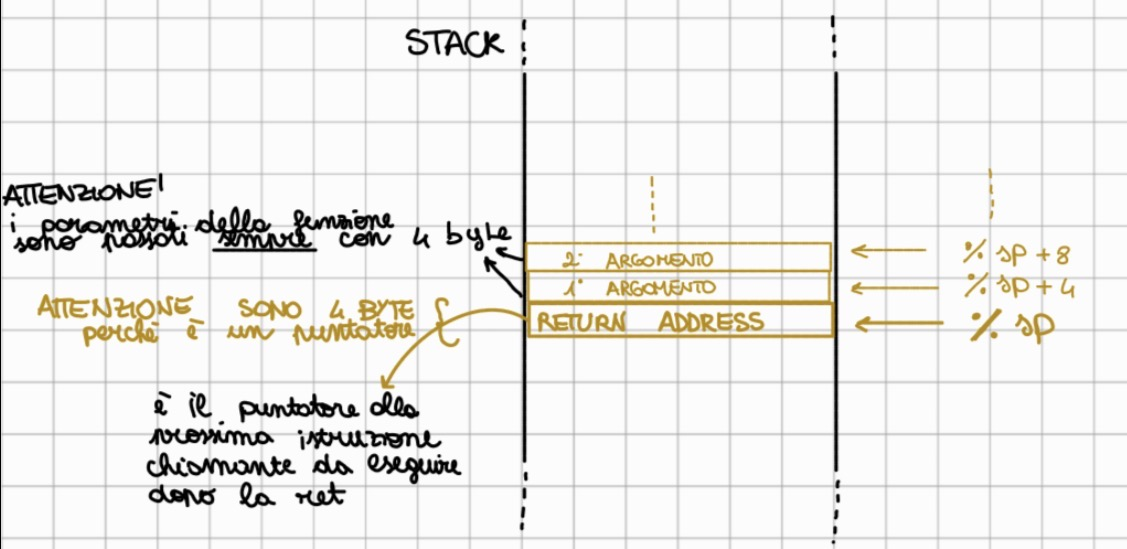
\includegraphics[width=0.7\linewidth]{../images/StackPointer2.jpg}
    \caption{StackPointer}
\end{figure}
\noindent\textcolor{red}{\textbf{Regola}:} tutti i parametri attuali (argomenti) occupano 4 byte ciascuno nello stack pointer indipendentemente dal loro tipo.
\subsection{Accesso in memoria con spiazzamento}
Per il "passaggio di parametri" in C, abbiamo l'equivalente in assembly in questo modo:
\begin{verbatim}
    d(addr) 
\end{verbatim}
dove \textit{d} indica lo spiazzamento e \textit{addr} è il puntatore a memoria. Nell'esempio precedente va applicato nel seguente modo:
\begin{verbatim}
    .globl f
    f:
        #a -> eax
        movl 4(%esp), %eax
        incl %eax
        ret
\end{verbatim}
Quindi avremo che nel registro eax sarà salvato il primo parametro passato dalla funzione. In generale avremo che:
\begin{verbatim}
    SP + 4 -> 4(%esp)
\end{verbatim}

\subsubsection{Operazioni aritmetico/logiche}
\begin{verbatim}
    add S, D | D <- D + S
    sub S, D | D <- D - S
    mul S, D | D <- D * S senza segno
   imul S, D | D <- D * S con segno
    and S, D | D <- D & S bit a bit
     or S, D | D <- D ^ S bit a bit
    xor S, D | D <- -D   viene utilizzato per l'inizializzazione delle variabili, 
                         preferito a movl poichè modifica i flag
    not S, D | D <- !D
    inc D    | D <- D + 1  
    dec D    | D <- D - 1
    neg D    | D <- -D
\end{verbatim}

\subsubsection{Moltiplicazione senza segno}
\begin{verbatim}
    mul S | D <- D * S 
            |    |   |
            |    |   |__ registro 32bit/immediato
     %edx:%eax  %eax   
\end{verbatim}
\noindent esempio:
\begin{verbatim}
                              eax          edx 
   movl $2, %eax            0....010        ?
                            
    mull $5                 0..01010     0......0
\end{verbatim}

\noindent \subsubsection{Moltiplicazione con segno}
\begin{verbatim}
   imul S | D <- D * S 
            |    |   |
            |    |   |__ registro 32bit/immediato
     %edx:%eax  %eax  
\end{verbatim}
\noindent esempio:
\begin{verbatim}
                              eax          edx 
   movl $-2, %eax            11....10        ?
                            
    imull $5                 1.......     11111111
\end{verbatim}

\subsubsection{Divisione}
\begin{verbatim}
    div S | D <- D / S
            |    |
            |    |
       eax,edx  eax:edx
                                            
    idivl r32/imm32 | eax <- edx:eax / S    // quoziente
                    | edx <- edx:eax % S    // modulo
\end{verbatim}

\section{Gestione del flusso di esecuzione}
\subsection{Salto incondizionato}
\begin{minipage}{0.4\textwidth}
\begin{verbatim}
...
...
goto L;
...
...
L:
...
...


c
\end{verbatim}
\end{minipage}
\hfill
$\longrightarrow$
\hfill
\begin{minipage}{0.4\textwidth}
\begin{verbatim}
...
...
jmp L
...
...
L:
...
...


Assembly
\end{verbatim}
\end{minipage}
\noindent

\subsection{Salto condizionato}
Le istruzioni di salto condizionato in ASM si sviluppano in due fasi:
\begin{enumerate}
    \item Esecuzione di istruzione aritmetico/logica che modifica EFLAGS
    \item Esecuzione di un salto condizionato al valore di EFLAGS
\end{enumerate}

\noindent La proprietà valutata in 2. per il salto è detta \textbf{condition code (cc)}
\\ esempio: 
\\ Risultato R

\begin{table}[H]
    
    \begin{tabular}{ccc}
        Condition Code (cc) & &Proprietà di R \\
        \hline
         e, z &  &R == 0 \\
         ne, nz &   &R != 0 \\     
        &Con segno: & \\
         g  &   &R $>$ 0\\
         l  &    & R $<$ 0\\
         ge &    & R $\ge$ 0\\
         le &    & R $\le$ 0\\
        &Senza segno: &\\
         a & & R $>$ 0 \\
         b &  &R $<$ 0 \\
         ae &  &R $\ge$ 0 \\
         be &  &  $\le$ 0 \\
         \hline
    \end{tabular}
\end{table}

\noindent Il salto condizionato è implementato da:
\begin{verbatim}
    jcc L
\end{verbatim}
\noindent esempio:
\begin{verbatim}
    subl %eax, %ecx     # R = ecx - eax
    je    L             # eax = ecx -> R==0
\end{verbatim}
\noindent esempio:
\begin{verbatim}
    subl %eax, %ecx     
    jge    L             # ecx >= eax -> R>=0
\end{verbatim}
\subsection{Registro EFLAGS}
È un registro contenente diversi flag (bit) dedicati a rappresentare lo stato della CPU a seguito dell'esecuzione dell'ultima istruzione:
\begin{figure} [H]
    \centering
    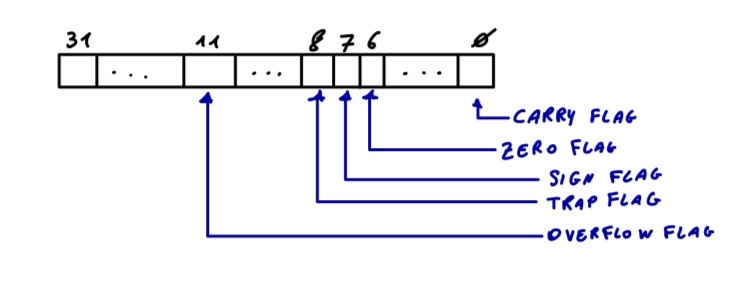
\includegraphics[width=0.6\linewidth]{../images/EFLAG.jpg}
    \caption{EFLAGS}
\end{figure}
\begin{itemize}
    \item \textbf{Bit 0} $\rightarrow$ il \textit{carry flag} serve principalmente a indicare un riporto (carry) o un prestito (borrow) nelle operazioni aritmetiche senza segno.
    \item \textbf{Bit 6} $\rightarrow$ la \textit{zero flag} ha come valore 1 se l'operazione precedente ha avuto come risultato zero, altrimenti varrà 0.
    \item \textbf{Bit 7} $\rightarrow$ il \textit{sign flag} quando l'operazione ha come risultato negativo vale 1 altrimenti 0 
    \item \textbf{Bit 8} $\rightarrow$ il \textit{trap flag} viene usato dal debugger
    \item \textbf{Bit 11} $\rightarrow$ l'\textit{overflow flag} indica quando si verifica un overflow nelle operazioni aritmetiche con numeri con segno. Questo succede quando il risultato non può essere rappresentato con il numero di bit disponibile.
\end{itemize}
7) 
8) usato dal debugger
11) per i risultati non rappresentabili nei nostri bit allora il flag varrà 1 

\section{Istruzioni di Condizione}
\medskip
\begin{minipage}{0.2\textwidth}
    \begin{verbatim}
        if(c>a){
            istr 1;
        }
        istr 2;
        
        f.c
    \end{verbatim}
\end{minipage}
\hfill
$\longrightarrow$
\hfill
\begin{minipage}{0.2\textwidth}
    \begin{verbatim}
        r = c - a;
        if(r<=0)goto L;
        istr 1;
        L:
            istr 2;
    
        f_eq.c
    \end{verbatim}
\end{minipage}
\hfill
$\longrightarrow$
\hfill
\begin{minipage}{0.2\textwidth}
    \begin{verbatim}
        subl %eax, %ecx
        jle L
        #istr 1
        L:
        #istr 2
        
        f.s
    \end{verbatim}
\end{minipage}\bigskip \\
\noindent In questo caso nel codice assembly abbiamo "sporcato" il registro \%ecx. Per non "sporcare" il registro con SUB usiamo \textit{CMP}, che ha la stessa funzione della sottrazione ma non salva in nessun registro.
\begin{verbatim}
    CMP S, D | D - S
\end{verbatim}
Ma altera i valori di EFLAGS esattamente come SUB. Avendo quindi un codice corretto in questo modo:\medskip\\
\begin{minipage}{0.3\textwidth}
    \begin{verbatim}
        if(test){
            blocco A;
        }else{
            blocco B;
        }
        blocco C;

        
        f.c
    \end{verbatim}
\end{minipage}
\hfill
$\longrightarrow$
\hfill
\begin{minipage}{0.3\textwidth}
    \begin{verbatim}
        if(!test)goto E;
        blocco A
        goto F;
        E:
            blocco B;
        F:
            blocco C;

    
        f_eq.c
    \end{verbatim}
\end{minipage}
\hfill
$\longrightarrow$
\hfill
\begin{minipage}{0.3\textwidth}
    \begin{verbatim}
        CMP S, D
        jcc E
        #blocco A
        jmp F
        E:
            #blocco B
        F:
            #blocco C
        
        f.s
    \end{verbatim}
\end{minipage}\bigskip\\
\noindent Inoltre esiste un'altra funzione simile chiamata \textit{Test} se dobbiamo fare una comparazione a 0, che è equivalente:
\begin{verbatim}
    cmp 0, D  | D - 0
    test D, D | D & D
\end{verbatim}

\subsection{Cicli While-For}
Vedremo ora come fare i cicli in Assembly, cominciando con il \textbf{\textit{while}}. Consideriamo lo schema generale dell'istruzione, se il test effettuato è vero, viene eseguito il blocco e si ritorna al test, altrimenti si prosegue con l'istruzione successiva al while, vediamo un esempio di traduzione in Assembly: \medskip\\ 
\begin{minipage}{0.2\textwidth}
    \begin{verbatim}
    while(test){
        blocco A;
    }
    blocco B;


    
    f.c
    \end{verbatim}
\end{minipage}
\hfill
$\longrightarrow$
\hfill
\begin{minipage}{0.2\textwidth}
    \begin{verbatim}
    L:
    if(!test) goto E;
    blocco A;
    goto L;
    E:
        blocco B


    f_eq.c
    \end{verbatim}
\end{minipage}
\hfill
$\longrightarrow$
\hfill
\begin{minipage}{0.2\textwidth}
    \begin{verbatim}
    L:
        cmp S, D
        jcc E
        blocco A
        jmp L
    E:
        blocco B
    
    f.s
    \end{verbatim}
\end{minipage}\medskip \\
\noindent Quindi non c'è una vera e propria traduzione in Assembly per il while ma occorrerà "smontare" il codice C, in un equivalente in grado di farci giostrare bene i jump, condizionali e non. Vediamo un esempio:\\
\begin{minipage}{0.2\textwidth}
    \begin{verbatim}
int sum(int n){
    int a = 0;
    int c = n;
    while(c>0){
        a = a + c;
        c--;
    }
    return a;
}



    
    f.c
    \end{verbatim}
\end{minipage}
\hfill
$\longrightarrow$
\hfill
\begin{minipage}{0.2\textwidth}
    \begin{verbatim}
int sum(int n){
    int a = 0;
    int c = n;
L:
    if(c<=0) goto E;
    a = a + c;
    c--;
    goto L;
E:
    return a;
}


    f_eq.c
    \end{verbatim}
\end{minipage}
\hfill
$\longrightarrow$
\hfill
\begin{minipage}{0.2\textwidth}
    \begin{verbatim}
.global sum
sum:
    xorl %eax, %eax
    movl 4(%esp), %ecx
L:
    testl $0, %ecx$
    jle E
    addl %ecx, %eax
    decl %ecx
    jmp L
E:
    ret

f.s
    \end{verbatim}
\end{minipage}\medskip \\
\noindent Consideriamo invece lo schema generale di una istruzione \textbf{\textit{for}}. Si segue dapprima l'inizializzazione e poi si effettua il test, se il test risulta vero allora viene eseguito il blocco, altrimenti si prosegue con l'istruzione successiva al for. In Assembly può essere tradotta in questo modo:\medskip\\
\begin{minipage}{0.4\textwidth}
    \begin{verbatim}
    for(init; test; update){
        blocco A
    }
    blocco B

    
    f.c
    \end{verbatim}
\end{minipage}
\hfill
$\longrightarrow$
\hfill
\begin{minipage}{0.4\textwidth}
    \begin{verbatim}
    init;
    while(test){
        blocco A
        update;
    }
    blocco B

    f_eq.c
    \end{verbatim}
\end{minipage} \medskip \\
\noindent Quindi passeremo dal for al while corrispondente che siamo già in grado di tradurre. Vediamolo meglio con un esempio: \medskip\\
\begin{minipage}{0.2\textwidth}
    \begin{verbatim}







    
unisigned fact(unisigned n){
    unisigned a = 1, c;
    for(c = 2; c<=n; c++)
        a*= c;
    return a;
}



    
    f.c
    \end{verbatim}
\end{minipage}
\hfill
$\longrightarrow$
\hfill
\begin{minipage}{0.2\textwidth}
    \begin{verbatim}
unisigned fact(unisigned n){
    unisigned a = 1;
    unisigned c;
    unisigned d = n;
    c = 2;
L:
    if(c>d) goto E;
    a = a * c;
    c++;
    goto L;
E:
    

    return a;
}


    f_eq.c
    \end{verbatim}
\end{minipage}
\hfill
$\longrightarrow$
\hfill
\begin{minipage}{0.2\textwidth}
    \begin{verbatim}
.globl fact
fact:
    movl $1, %eax
    movl $2, %ecx
    movl 4(%esp), %edx
L:
    cmpl %edx, %ecx
    # poichè senza segno 
    # usiamo ja e non jcc
    ja E      
    imull %ecx, %eax
    incl %ecx
    jmp L
E:
    ret

    
    f.s
    \end{verbatim}
\end{minipage}\medskip \\
\noindent Quindi per un ciclo for procederemeo in questo modo: \textit{for} $\rightarrow$ \textit{while} $\rightarrow$ \textit{if}.

\section{Puntatori}
Un puntatore in C di tipo \textit{T*} contiene un indirizzo di memoria dove è conservato un valore di \textit{tipo T}. In Assembly per indirizzare una locazione di memoria il cui indirizzo è contenuto in un registro usiamo l'operatore '\textbf{()}'.
\begin{minipage}{0.4\textwidth}
    \begin{verbatim}
    int *a;
    .
    .
    .
    *a = 0;

    
    f.c
    \end{verbatim}
\end{minipage}
\hfill
$\longrightarrow$
\hfill
\begin{minipage}{0.4\textwidth}
    \begin{verbatim}
    #int *a -> eax
    .
    .
    .
    movl $0, (%eax)

    f.s
    \end{verbatim}
\end{minipage} \medskip \\
\noindent Vediamolo in modo grafico:
\begin{figure} [H]
    \centering
    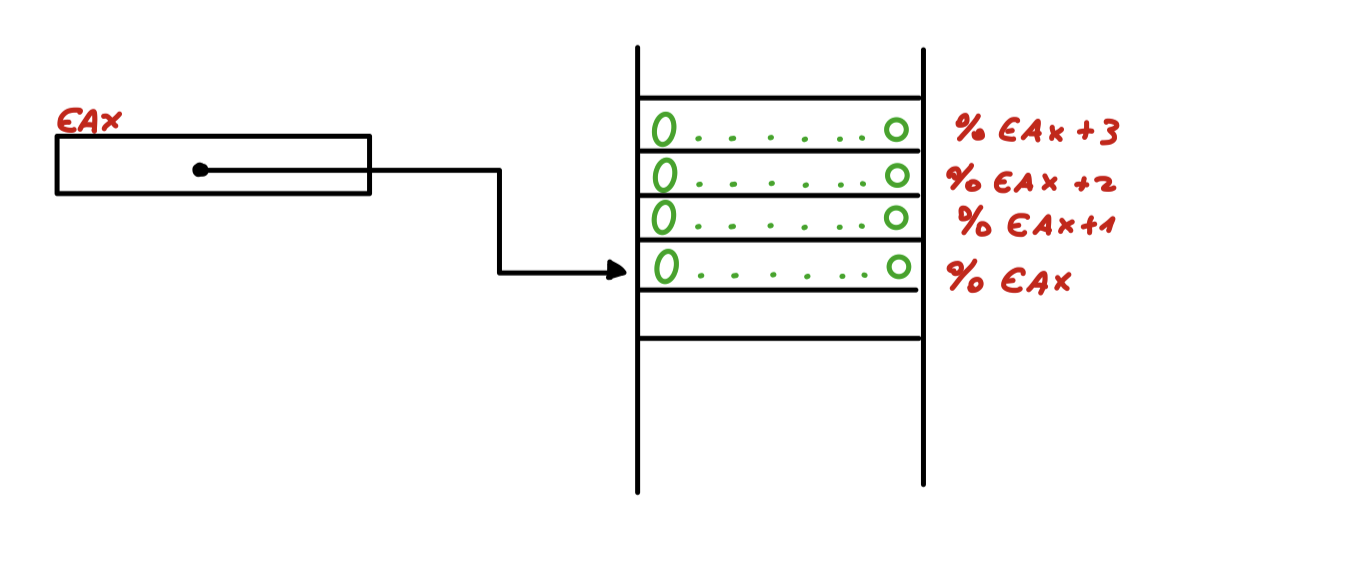
\includegraphics[width=0.7\linewidth]{../images/Puntatore EAX.png}
    \caption{Come occupa EAX la memoria in caso di int}
\end{figure}
\noindent Inoltre vale anche: int c = *a; $\rightarrow$ movl(\%eax), \%ecx\\
Nel caso dei puntatori la "l" del tipo di dato dipende dalla dimensione del tipo del puntatore (sizeof(T)). Esempio:\medskip\\
\begin{minipage}{0.4\textwidth}
    \begin{verbatim}
    char *p;
    .
    .
    .
    char a = *0;

    
    f.c
    \end{verbatim}
\end{minipage}
\hfill
$\longrightarrow$
\hfill
\begin{minipage}{0.4\textwidth}
    \begin{verbatim}
    #char *p -> edx
    .
    .
    .
    movb (%edx), %eax

    f.s
    \end{verbatim}
\end{minipage} \medskip \\
Quando accediamo al parametro passato per valore ad una funzione, stiamo in effetti usando un puntatore con l'operando '()'. Per capirci meglio: \medskip\\
\begin{minipage}{0.4\textwidth}
    \begin{verbatim}
    void f(int x){
        int a = x;
    }

    
    f.c
    \end{verbatim}
\end{minipage}
\hfill
$\longrightarrow$
\hfill
\begin{minipage}{0.4\textwidth}
    \begin{verbatim}
    movl 4(%esp), %eax

    f.s
    \end{verbatim}
\end{minipage} \medskip \\
\noindent In questi casi noi abbiamo sempre usato dei puntatori verso lo stackpointer:
\begin{figure} [H]
    \centering
    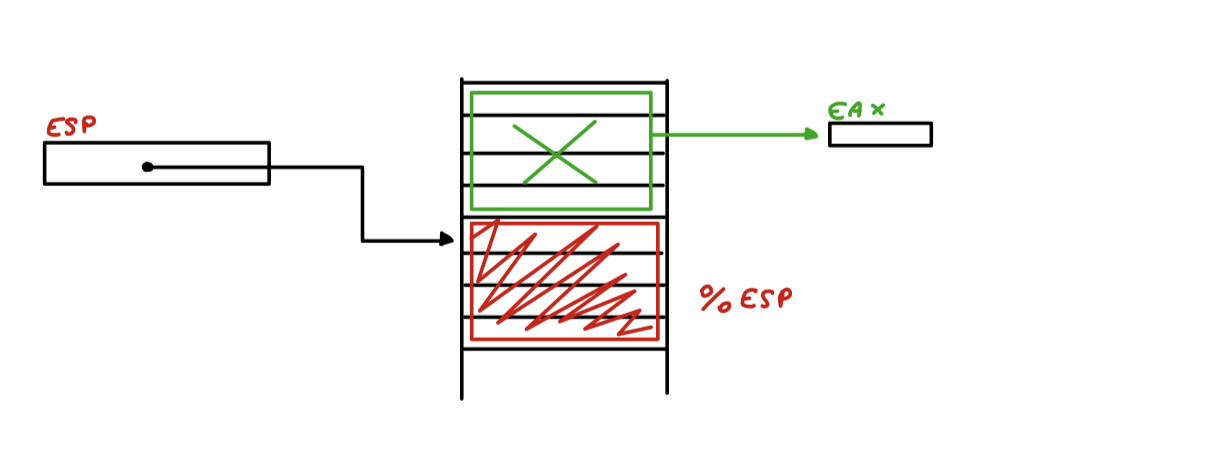
\includegraphics[width=0.7\linewidth]{../images/Funzionamento Memoria con ESP.png}
    \caption{Memoria Graficamente}
\end{figure}
\noindent Con lo stesso ragionamento possiamo capire come tradurre gli array in Assembly, molto semplicemente basta accedere alla posizione di memoria corrispondente alla posizione dell'array: \medskip\\
\begin{minipage}{0.4\textwidth}
    \begin{verbatim}
    int a[7] = 12;

    f.c
    \end{verbatim}
\end{minipage}
\hfill
$\longrightarrow$
\hfill
\begin{minipage}{0.4\textwidth}
    \begin{verbatim}
    movl $12, 28(%eax)

    f.s
    \end{verbatim}
\end{minipage} \medskip \\
\noindent Vediamolo meglio però con un esempio: \medskip \\
\begin{minipage}{0.4\textwidth}
    \begin{verbatim}
    void f(char *x){
        char c = x[1];
    }
    
    f.c
    \end{verbatim}
\end{minipage}
\hfill
$\longrightarrow$
\hfill
\begin{minipage}{0.4\textwidth}
    \begin{verbatim}
    movb 4(%esp), %eax
    movb 1(%eax), %ecx


    f.s
    \end{verbatim}
\end{minipage} \medskip \\
\noindent \textcolor{red}{\textbf{Importante:}} in una istruzioe IA32 è possibile l'accesso a memoria per al più un operando, inoltre l'operatore '()' può essere usato solo sui registri e questi registri devono contenere indirizzi validi di memoria. \\
Vediamo il tutto con un esempio: \medskip \\
\begin{minipage}{0.2\textwidth}
    \begin{verbatim}
void times2(short *p){
    *p = *p * 2;
}








    f.c
    \end{verbatim}
\end{minipage}
\hfill
$\longrightarrow$
\hfill
\begin{minipage}{0.2\textwidth}
    \begin{verbatim}
void times2(short *p){
    short *a = p;
    short cx = *a;
    *a = cx;
}







    f_eq.c
    \end{verbatim}
\end{minipage}
\hfill
$\longrightarrow$
\hfill
\begin{minipage}{0.2\textwidth}
    \begin{verbatim}
.globl times2
times2:
    movb 4(%esp), %eax
    #essendo short non c'è
    #bisogno della 'e'
    movw (%eax), %cx
    #equivalente fare:
    #imulw $2, %ecx
    addw $cx, $cx
    movw $cx, (%eax)
    ret

    f.s
    \end{verbatim}
\end{minipage}\medskip \\
\subsection{Accesso in memoria con base,indice e spiazzamento}
D(x) $\rightarrow$ accede alla locazione con indirizzo x + D, in realtà la sintassi completa dell'operatore '()' è: 
\begin{verbatim}
    imm(base,indice,scala)
\end{verbatim}
\noindent dove:
\begin{itemize}
    \item \textit{imm} $\rightarrow$ rappresetna lo spiazzamento definito come valore costante
    \item \textit{base} $\rightarrow$ è l'indirizzo di memoria di base a cui deve accedere. \textbf{DEVE} essere un registro e \textbf{DEVE} essere valido
    \item \textit{indice} $\rightarrow$ indice dell'elemento a cui si vuole accedere a partire da BASE e \textbf{DEVE} essere un registro opzionale
    \item \textit{scala} $\rightarrow$ dimensione in byte di ogni elemento. \textbf{DEVE} essere un valore costante: 1,2,4 ed 8 (l'8 solo a 64 bit). Ed è opzionale
\end{itemize}
\noindent L'uso dell'operatore permette di accedere alla memoria con \textbf{indirizzo} $\rightarrow$ Base + Indice $\times$ Scala + Imm\\
Esempio: \medskip \\ 
\begin{minipage}{0.4\textwidth}
    \begin{verbatim}
    int a[7] = 12;




    f.c
    \end{verbatim}
\end{minipage}
\hfill
$\longrightarrow$
\hfill
\begin{minipage}{0.4\textwidth}
    \begin{verbatim}
    movl $7, %ecx
    movl $12, (%eax, %ecx, 4)
    # corrisponde a 
    # movl $12, 28(%eax)
    
    f.s
    \end{verbatim}
\end{minipage} \medskip \\
\noindent Vediamo un esempio con un codice in C: \medskip\\
\begin{minipage}{0.2\textwidth}
    \begin{verbatim}
short get(short* v, 
    unsigned n, unsigned i){
    if(i>=n) return -1;
    return v[i];
}








    f.c
    \end{verbatim}
\end{minipage}
\hfill
$\longrightarrow$
\hfill
\begin{minipage}{0.2\textwidth}
    \begin{verbatim}
short get(short* v, 
    unsigned n, unsigned i){
    short *c = v;
    unsigned d = i;
    unsigned a = n;
    short ax;
    if(d<a) goto E;
    ax = -1;
    return ax;
    E:
        ax = c[d];
        return ax;
}

    f_eq.c
    \end{verbatim}
\end{minipage}
\hfill
$\longrightarrow$
\hfill
\begin{minipage}{0.2\textwidth}
    \begin{verbatim}
.globl get
get:
    movl 4(%esp), %ecx
    movl 12(%esp), %edx
    movl 8(%esp), %eax
    cmpl %eax, %edx
    jb E
    movlw $-1, %ax
    ret
    E:
    movw (%ecx,%edx,2), %ax
    ret
    

    f.s
    \end{verbatim}
\end{minipage}\medskip \\
\noindent Il tipo del puntatore definisce inoltre il valore da aggiungere all’indirizzo base. Inoltre opereremo su puntatori \textbf{sempre} con operatori a 4 byte. In C esiste un’aritmetica dei puntatori \textbf{implicita}, ovvero non dobbiamo preoccuparci di dove puntano i puntatori; mentre in Assembly l’aritmetica dei puntatori è \textbf{esplicita}.
\begin{figure}[H]
    \centering
    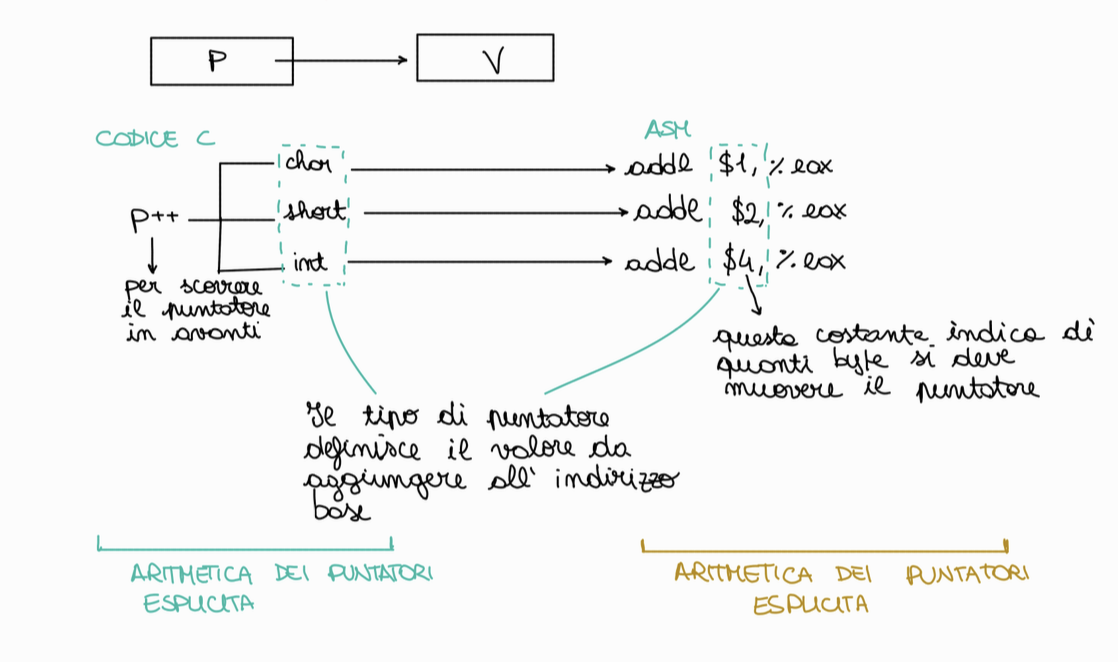
\includegraphics[width=0.5\linewidth]{../images/Aritmetica Puntatore.png}
    \caption{Puntatore}
\end{figure}

\section{Chiamate a Funzione}
\begin{figure}[H]
    \centering
    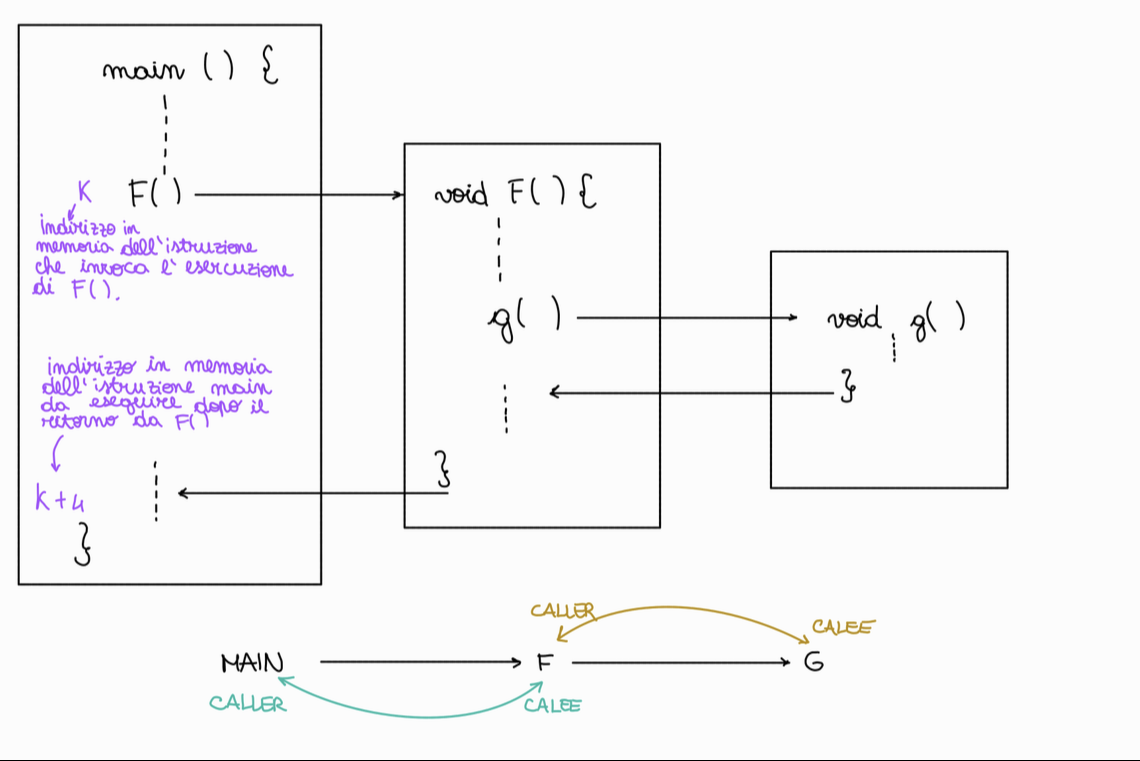
\includegraphics[width=0.5\linewidth]{../images/Chiamata a funz.png}
    \caption{Chiamata a funzione}
\end{figure}
\noindent In questo esempio cominciamo definendo queste funzioni. Avremo che il main sarà il nostro \textbf{caller}, mentre f sarà il \textbf{callee}. Tuttavia, anche tra f e g esiste una relazione: in questo caso f sarà il \textbf{caller}, mentre g il \textbf{callee}. Quindi una funzione può assumere ruoli diversi a seconda del rapporto che ha con le altre funzioni. \\
La stack è fondamentale per gestire le chiamate a funzione e per fornire spazio di memoria locale. Ogni chiamata a funzione crea uno \textbf{stack frame} (o record di attivazione), che contiene variabili locali, parametri e altre informazioni necessarie all’esecuzione della funzione.
Gli stack frame sono organizzati come una sorta di \textbf{lista collegata}: il registro ebp punta allo \textbf{stack frame} della funzione attualmente in esecuzione, e ogni frame contiene un riferimento a quello della funzione chiamante. Questo permette, ad esempio, a un debugger di ricostruire la sequenza di chiamate dal main fino alla funzione corrente. Tuttavia, il collegamento tra \textbf{stack frame} tramite ebp è \textbf{opzionale}. \\
\noindent\textbf{\textcolor{red}{Importante:}} per convenzione, nel momento in cui si effettua un’istruzione CALL, la base della stack puntata dal registro \%esp deve essere sempre a un indirizzo multiplo di 16.
\begin{figure} [H]
    \centering
    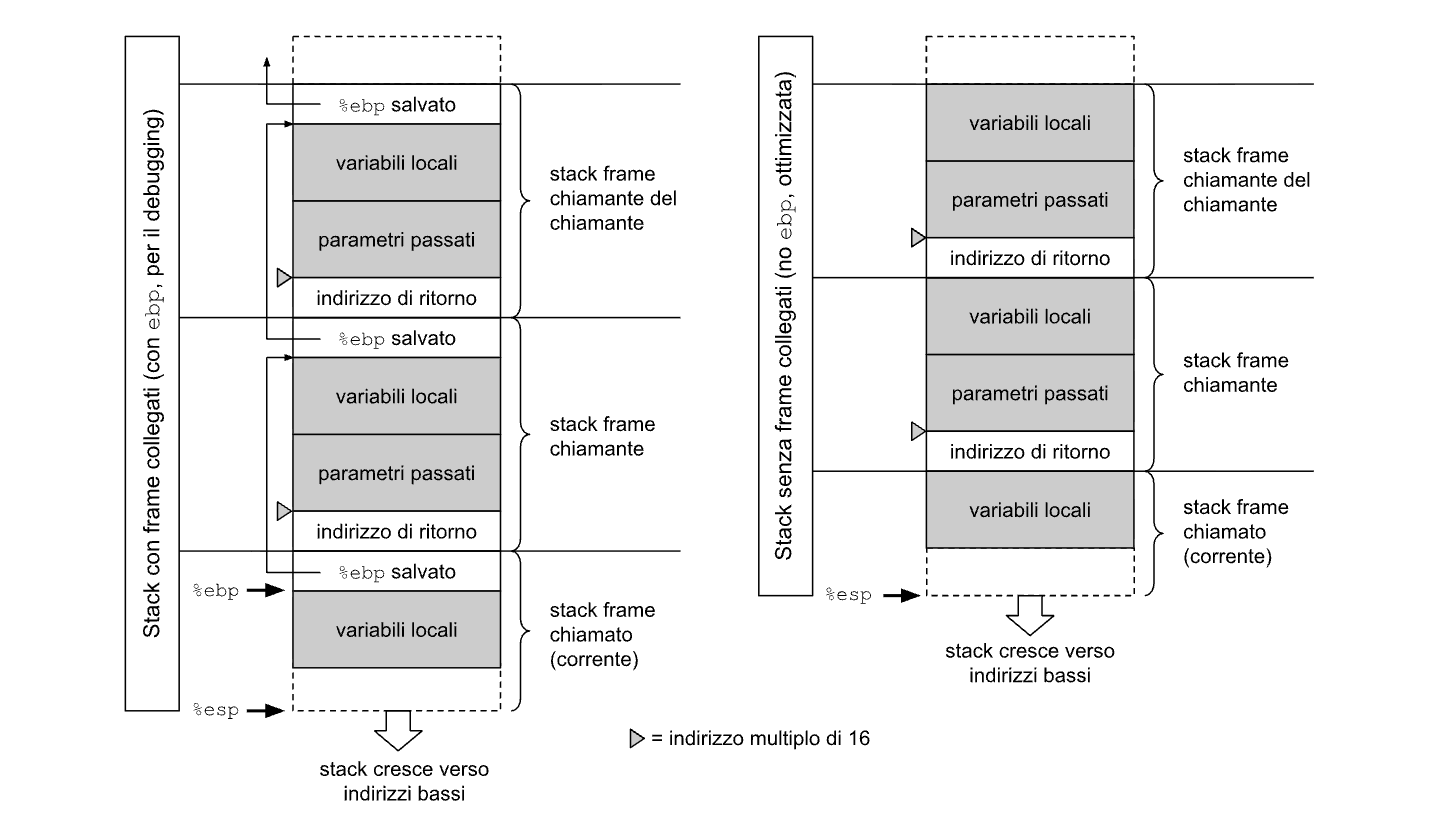
\includegraphics[width=0.7\linewidth]{../images/Funzione Stack Pointer.png}
    \caption{Stack Pointer specifico alle funzioni}
\end{figure} 
\noindent Vediamo però cosa può contenere il frame/record di attivazione di una funzione:
\begin{itemize}
    \item Variabili locali
    \item Copie dei registri $\rightarrow$ ebx, edi, esi, ebp
    \item Parametri per le funzioni chiamate
    \item Indirizzo di ritorno delle funzioni chiamate
\end{itemize}
\begin{figure} [H]
    \centering
    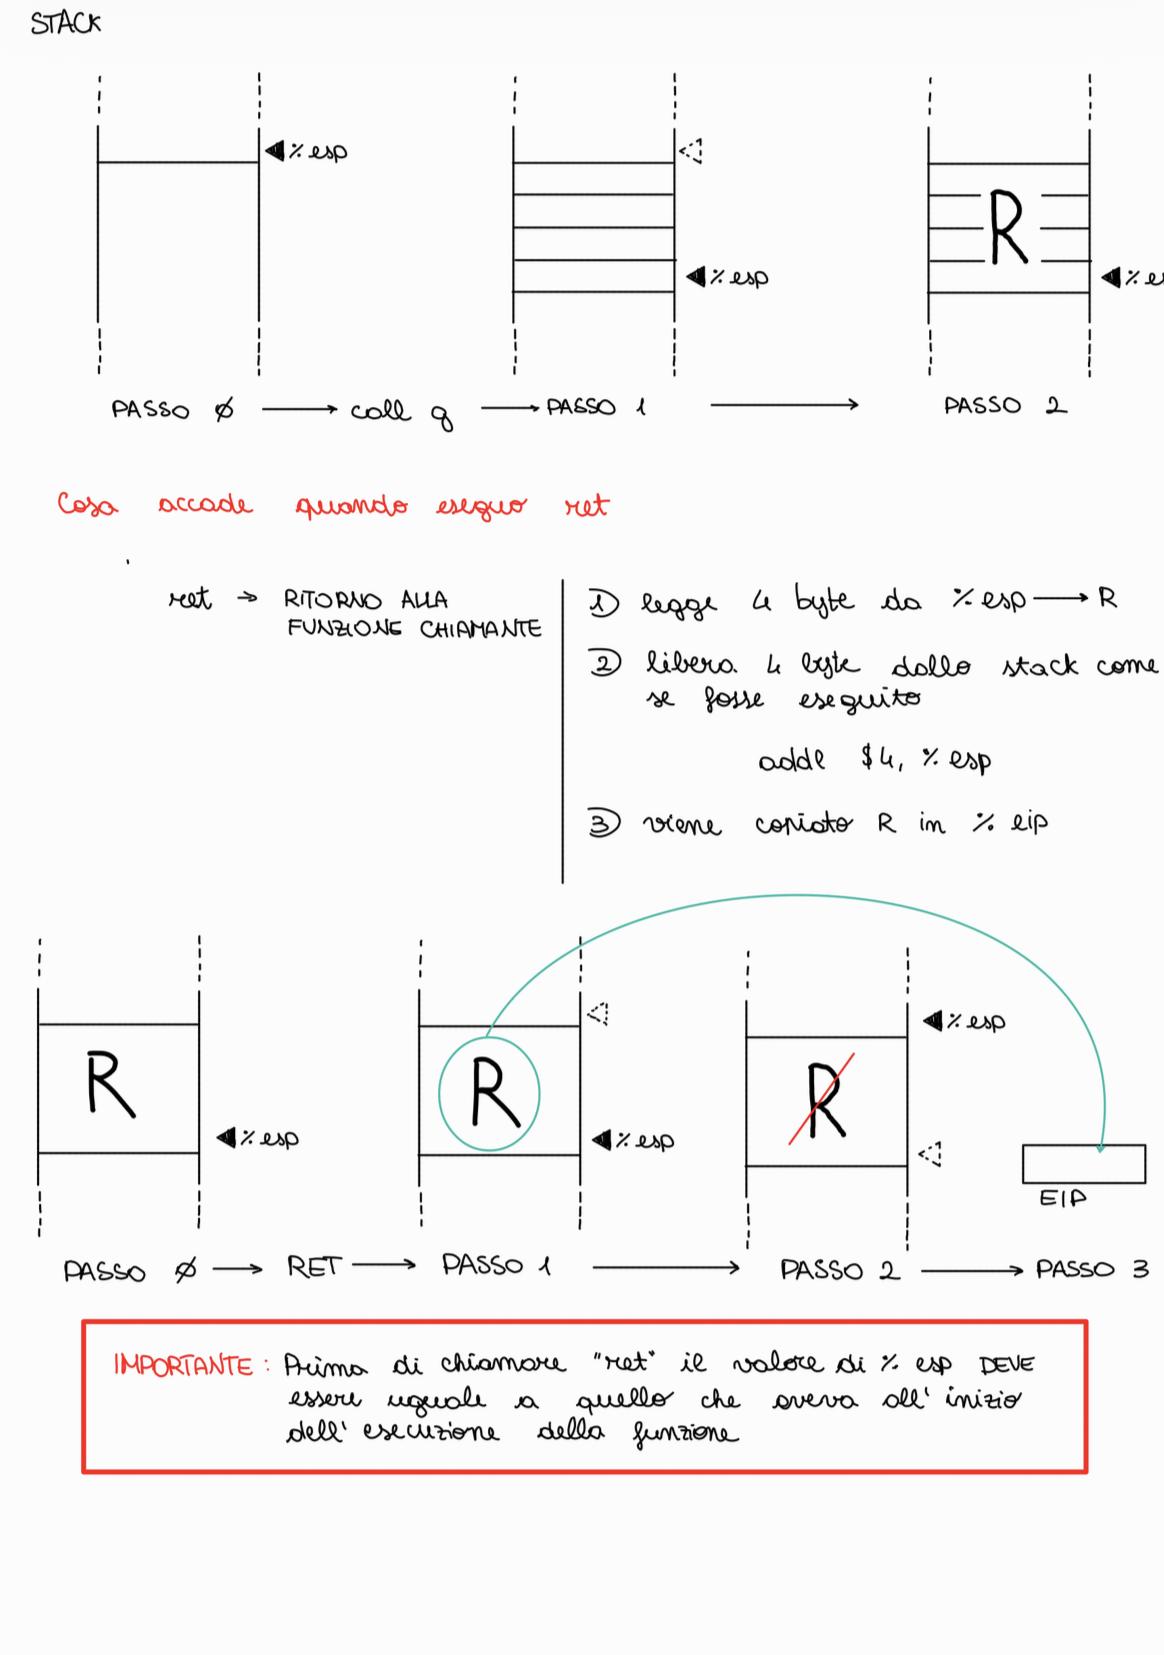
\includegraphics[width=0.4\linewidth]{../images/Ret cosa accade.png}
    \caption{Cosa accade quando utilizziamo il ret?}
\end{figure}

\noindent \textcolor{red}{\textbf{Importante:}} prima di chiamare ret il valore \%esp deve essere uguale a quello che aveva all'inizio dell'esecuzione  \medskip \\
\begin{minipage}{0.2\textwidth}
    \begin{verbatim}
int f(){
    int a = 1 + g();
    //g è definita nel main 
    //che qui non scriviamo
    //g () { return 10 }
    return a;
}

    f.c
    \end{verbatim}
\end{minipage}
\hfill
$\longrightarrow$
\hfill
\begin{minipage}{0.2\textwidth}
    \begin{verbatim}
int f(){
    int a;
    a = g(); 
    a = a + 1;
    return a;
}

    f_eq.c
    \end{verbatim}
\end{minipage}
\hfill
$\longrightarrow$
\hfill
\begin{minipage}{0.2\textwidth}
    \begin{verbatim}
.globl f
f:
    #e -> eax
    call g
    #il valore è gia in eax
    #essendo il ret di g
    incl %eax
    ret
    
    f.s
    \end{verbatim}
\end{minipage}\medskip \\
\noindent Vediamo invece cosa accade nello Stack Pointer quando abbiamo un passaggio di parametri
\begin{figure} [H]
    \centering
    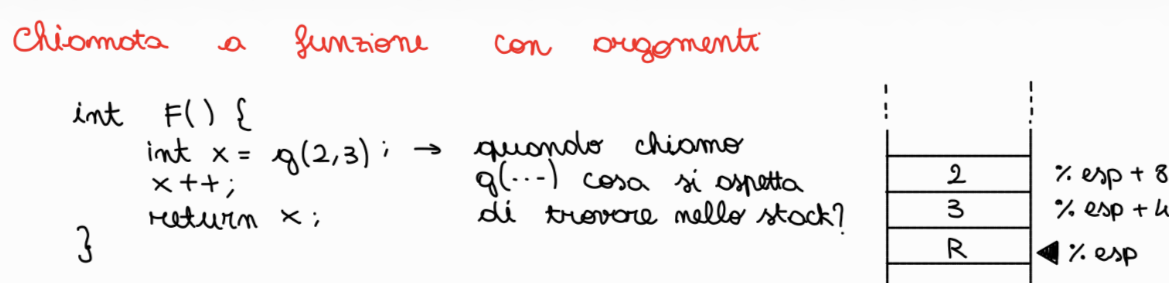
\includegraphics[width=0.5\linewidth]{../images/passaggio parametri sp.png}
    \caption{Passaggio parametri}
\end{figure} 
\noindent Quindi avremo che lo SP:
\begin{enumerate}
    \item Riserva spazio per i parametri come se fosse: \texttt{subl \$8, \%esp} , dove 8 è uguale al numero di parametri passati per 4 (spazio occupato in memoria)
    \item Copia i valori attuali dei parametri nello spazio riservato in ordine inverso
    \item Chiamata di funzione: call g
\end{enumerate}
\begin{minipage}{0.4\textwidth}
    \begin{verbatim}
    




int f(){
    int x = g(2,3);
    //g è definita nel main 
    //che qui non scriviamo
    x++;
    return x;
}





    f.c
    \end{verbatim}
\end{minipage}
\hfill
$\longrightarrow$
\hfill
\begin{minipage}{0.4\textwidth}
    \begin{verbatim}
.globl f
f:
    #8 perchè 4 * 2 parametri
    subl $8, %esp       #prologo
    #scrivo i parametri attuali
    #nello spazio che ho riservato
    movl $3, 4(%esp)
    movl $2, 8(%esp)
    call g
    #dato che se g restituisce qualcosa
    #lo restituisce in eax avremo
    #eax già modificato
    incl %eax
    #riportiamo %esp al valore "originale"
    addl $8, %esp       #epilogo
    ret
    
    
    f.s
    \end{verbatim}
\end{minipage}\medskip \\
\begin{figure}[H]
    \centering
    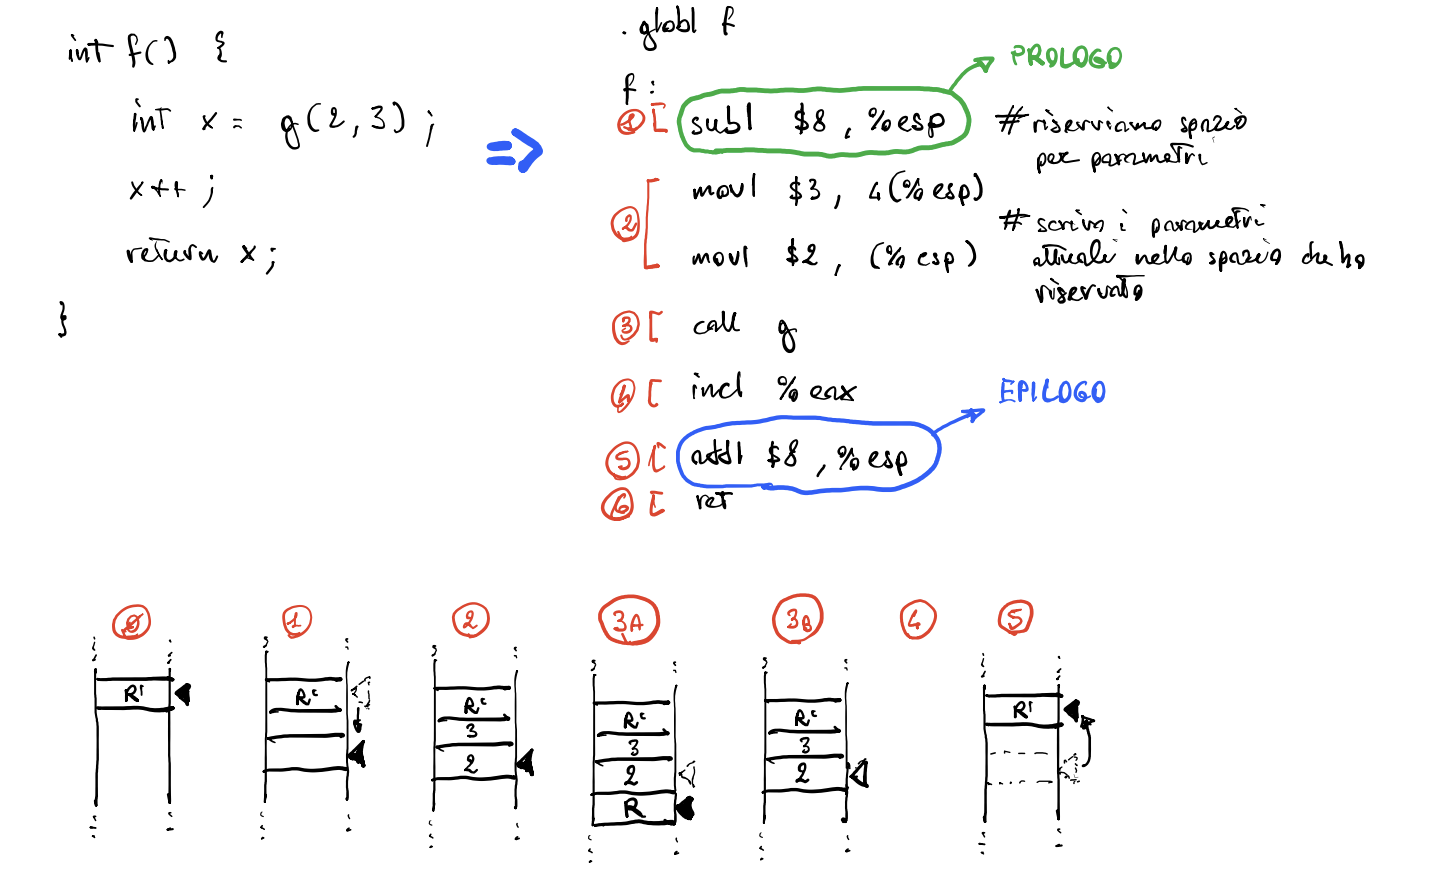
\includegraphics[width=0.9\linewidth]{../images/Esempio Grafico programma.png}
    \caption{Struttura del codice}
\end{figure}
\noindent La lista di stack frame viene gestita mediante un codice di \textbf{prologo} all’inizio di una funzione e un codice di \textbf{epilogo} alla fine:
\begin{itemize}
    \item \textit{prologo} $\rightarrow$ salva nello stack il contenuto del registro \textbf{ebp}, che punta allo stack frame del chiamante, tramite l’istruzione \texttt{pushl \%ebp}. Successivamente il registro \textbf{ebp} viene aggiornato per puntare alla posizione corrente dello stack, contenuta nel registro \textbf{esp}, mediante l’istruzione \texttt{movl \%esp, \%ebp}. In questo modo \textbf{ebp} viene a puntare allo stack frame della funzione corrente.
    \item \textit{epilogo} $\rightarrow$ ripristina il valore del registro \textbf{ebp} presente prima dell’attivazione della funzione corrente eseguendo l’istruzione \texttt{popl \%ebp}. In questo modo \textbf{ebp} tornerà a puntare allo stack frame della funzione chiamante.
\end{itemize}
\noindent In gcc, è possibile omettere il collegamento fra stack frame compilando con l’opzione -fomit-frame-pointer. In questo modo, non verranno generati prologo ed epilogo: la funzione sarà più veloce e compatta, ma il debugging potrebbe essere più difficoltoso.\medskip\\ 
L’esecuzione di una funzione può sovrascrivere i registri utilizzati dal chiamante. Se il chiamante vuole garantire che il contenuto di un registro non venga modificato durante l’invocazione di una funzione, è necessario salvarne il valore da qualche parte, generalmente nello stack. Esistono due possibili strategie:
\begin{enumerate}
    \item \textbf{caller-save}: il registro viene salvato nello stack dal chiamante prima dell’invocazione della funzione e ripristinato subito dopo il ritorno. La funzione chiamante (caller) deve salvare il valore di questi registri prima di chiamare un'altra funzione. La funzione chiamata invce può modificare liberamente il valore di questi registri.
    \item \textbf{callee-save}: il registro viene salvato nello stack dal chiamato prima di eseguire il corpo della funzione e ripristinato prima di ritornare al chiamante. La funzione chiamata (callee) deve preservare il valore che questi registri riservano nel momento in cui viene eseguita la call, e deve ripristinarli prima di eseguire il ret (il salvataggio avviene nel prologo e il ripristino nell’epilogo).
\end{enumerate}
Per convenzione, alcuni registri vengono salvati dal chiamante, e altri dal chiamato:
\begin{itemize}
    \item \textbf{Registri caller-save} $\rightarrow$ A, C, D.
    \item \textbf{Registri callee-save} $\rightarrow$ B, DI, SI, SP, BP.
\end{itemize}
Ma come si salva il valore di un registro?
\begin{enumerate}
    \item Salviamo il valore di \texttt{\%reg} (registro qualsiasi) nella stack
    \item Eseguiamo le operazioni che "cambiano" il contenuto di \%reg
    \item Recuperiamo dalla stack il valore di \%reg
\end{enumerate}
Ci sono diversi modi per farlo, vediamo il \textit{modo esplicito}:
\begin{verbatim}
1)  subl $4, %esp
    movl %reg, (%esp)
2)  #%reg viene sporcato
3)  movl (%esp), %reg
    addl $4, (%esp)
\end{verbatim}
\noindent \subsection{Metodo \textit{Push + Pop}}
\begin{verbatim}
1)  push %reg
2)  # . . .
3)  popl %reg
\end{verbatim}
In questi due metodi abbiamo che l'1) e il 3) sono equivalenti tra loro quindi possiamo usare entrambi a nostro piacimento. \medskip\\
\begin{minipage}{0.2\textwidth}
    \begin{verbatim}
    



int f(){
    return g() + h();
}



    f.c
    \end{verbatim}
\end{minipage}
\hfill
$\longrightarrow$
\hfill
\begin{minipage}{0.2\textwidth}
    \begin{verbatim}
int f(){
    int a; 
    a = g();
    int c;
    c = a;
    a = h();
    a = a + c;
    return a;
}

    f_eq.c
    \end{verbatim}
\end{minipage}
\hfill
$\longrightarrow$
\hfill
\begin{minipage}{0.2\textwidth}
    \begin{verbatim}
.globl f
f:
    #a -> EAX
    #c -> ECX
    call g 
    movl %eax, %ecx
    pushl %ecx
    call h
    popl %ecx
    addl %ecx, %eax
    ret
    
    f.s
    \end{verbatim}
\end{minipage}\medskip \\
Avremmo potuto usare anche il metodo esplicito ed avremmo avuto lo stesso identico risultato.\\
Vediamo però che registri usare a seconda delle situazioni:
\begin{itemize}
    \item Se implemento una funzione che \textbf{NON} chiama altre funzioni:
    \begin{itemize}
        \item uso liberamente i caller saved (A, C, D).
        \item  se non sono sufficienti allora uso i callee saved (B, DI, SI, BP) ma preservando il valore (usando prologo + epigolo).
    \end{itemize}
    \item Se implemento una funzione che chiama altre funzioni:
    \begin{itemize}
        \item Uso i callee saved (B, DI, SI, BP) preservandone il valore
        \item Uso liberamente i caller saved (A, C, D) per valori temporanei \textbf{SOLO} in blocchi di istruzioni che \textbf{NON} chiamano altre funzioni,
        \item Altrimenti uso i caller saved (A, C, D) ma ne preservo il valore (push + pop) prima di \textbf{QUALSIASI} chiamata a funzione.
    \end{itemize}
\end{itemize}
\begin{minipage}{0.2\textwidth}
    \begin{verbatim}
int g(int x);

int f(){
    int y = 1, z = 2;
    return g(x+1) + y + z;
}















    f.c
    \end{verbatim}
\end{minipage}
\hfill
$\longrightarrow$
\hfill
\begin{minipage}{0.2\textwidth}
    \begin{verbatim}
int f(){
    int c;
    int di; // y
    int si; // z
    c = x;
    di = 1;
    si = 2;
    c++;
    int a = g(c);
    a = a+di;
    a = a + si;
    return a;
}








    f_eq.c
    \end{verbatim}
\end{minipage}
\hfill
$\longrightarrow$
\hfill
\begin{minipage}{0.3\textwidth}
    \begin{verbatim}
.globl f
f:
    #Prologo
    pushl %edi # -> y
    pushl %esi # -> z
    subl $4, (%esp)
    
    movl 16(%esp), %ecx
    movl $1, %edi
    movl $2, %esi
    incl %ecx
    movl %ecx, (%esp)
    call g
    addl %edi, %eax
    adll %esi, %eax
    #Epilogo
    addl $4, (%esp)
    popl %edi
    popl %esi
    ret
    
    f.s
    \end{verbatim}
\end{minipage}\medskip \\
\begin{figure} [H]
    \centering
    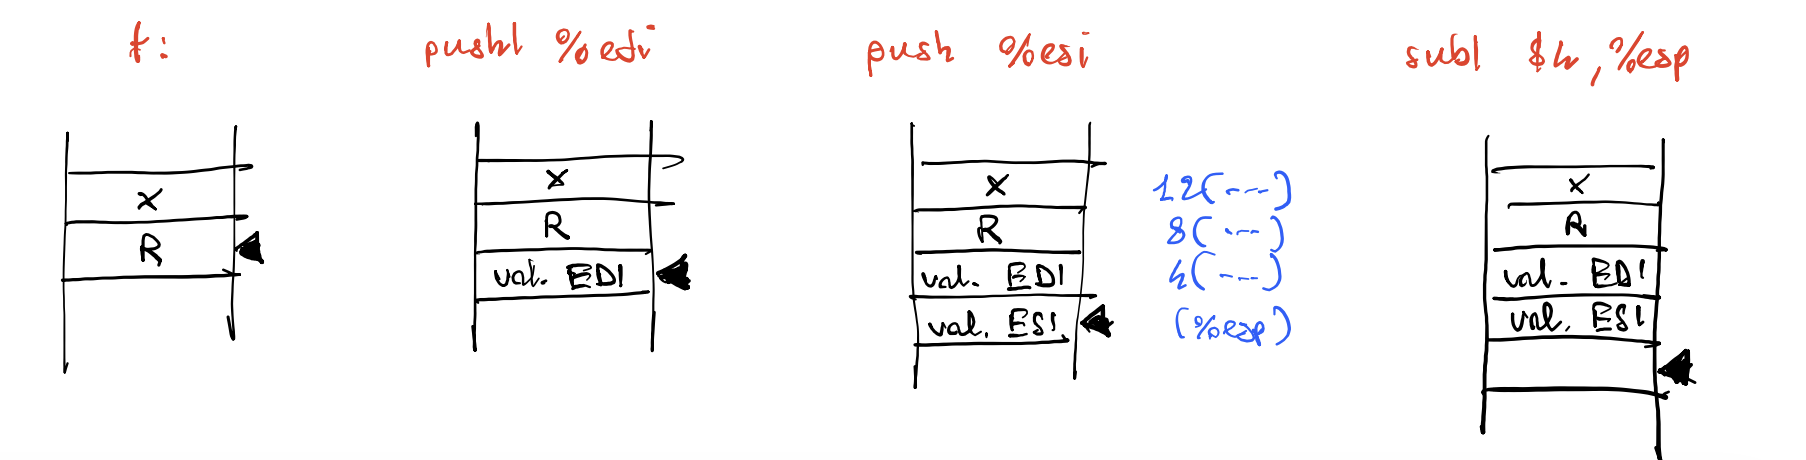
\includegraphics[width=0.9\linewidth]{../images/Graficamente nello SP.png}
    \caption{Graficamente}
\end{figure}
\newpage
Esercizio riassuntivo su quello fatto fino ad ora: \medskip\\
% PRIMO BLOCCO (da solo sopra)
\begin{center}
\begin{minipage}{0.4\textwidth}
\begin{verbatim}
int is_negative(int x);

int f(int *v, unsigned n){
    unsigned i, cnt = 0;
    for(i = 0; i < n; i++){
        cnt += is_negative(v[i]);
    }
    return cnt;
}

f.c
\end{verbatim}
\end{minipage}
\end{center}

\vspace{1cm}

% SECONDA RIGA (due blocchi affiancati)
\noindent
\begin{minipage}{0.45\textwidth}
\begin{verbatim}
int f(int *v, unsigned n){
    int *di = v;
    unsigned si = n;
    unsigned b = 0;
    unsigned bp = 0;
L:
    if(b >= si) goto E;
    int c = di[b];
    unsigned a = is_negative(c);
    bp = bp + a;
    b++;
    goto L;
E:
    a = bp; 
    return a;
}

f_eq.c
\end{verbatim}
\end{minipage}
\hfill
$\longrightarrow$
\hfill
\begin{minipage}{0.45\textwidth}
\begin{verbatim}
.globl f
f:
    pushl %edi
    pushl %esi
    pushl %ebx
    pushl %ebp
    subl $4, %esp

    movl 24(%esp), %edi
    movl 28(%esp), %esi
    xorl %ebx, %ebx
    xorl %ebp, %ebp
L:
    cmpl %esi, %ebx
    jae E
    movl (%edi,%ebx,4), %ecx 
    #4 * ebx (=i) quindi muove di 4 * i %edi 
    #per prendere tutti i valori del vettore
    movl %ecx, (%esp)
    call is_negative
    addl %eax, %ebp
    incl %ebx
    jmp L
E:
    movl %ebp, %eax
    ret
\end{verbatim}
\end{minipage}

\newpage
\section{Conversione del tipo (cast)}
Partiamo dal fatto che in Assembly il cambio di tipo, così come lo intendiamo nei linguaggi ad alto livello, non esiste. In questo contesto dobbiamo invece distinguere due casi principali:

\begin{enumerate}
    \item \textbf{Operazioni di troncamento (downcast)} $\rightarrow$ ad esempio: \texttt{int c = 0x000CAFE} (32 bit) $\rightarrow$ \texttt{char a = c} (8 bit).  
    In questo caso si mantengono solo i bit meno significativi, con conseguente perdita di informazione. % METTERE IL DISEGNO DI GIO DAJE ROMA DAJE  
    (Esempio implementabile con istruzioni come \texttt{movl}).

    \item \textbf{Operazioni di promozione (upcast)} $\rightarrow$ in questo caso il valore viene esteso a un tipo più grande.  
    È importante distinguere tra estensione con segno e senza segno, a seconda che il dato originale sia signed oppure unsigned.
    \begin{verbatim}
                    con     |   char c='s';             8 bit
                    segno   |   int a=c;                32 bit
                
                    senza   |   unsigned char c='s';    8 bit
                    segno   |   unsigned int a=c;       32 bit
    \end{verbatim}  
    Con questo tipo di operazione non si ha perdita di informazione, a differenza del downcast. Tuttavia, è necessario garantire esplicitamente che il segno venga preservato.
    \begin{figure} [H]
        \centering
        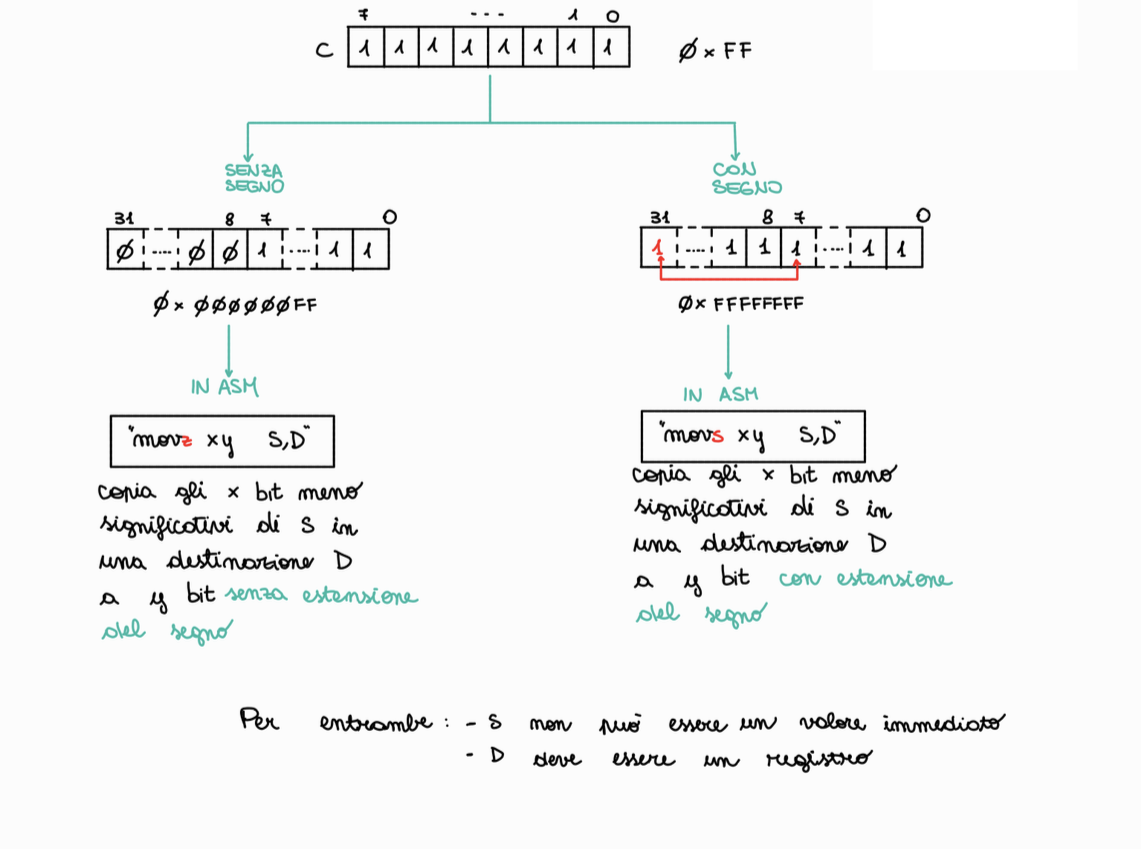
\includegraphics[width=0.9\linewidth]{../images/Segno Char Int.png}
        \caption{Estensione con segno da \texttt{char} a \texttt{int}}
    \end{figure}
    
    Nel caso di una promozione da \texttt{char} a \texttt{int}, per preservare il segno è necessario propagare il bit più significativo del \texttt{char} (bit di segno) su tutti i bit aggiuntivi dell'\texttt{int}.  
    
    Per questo motivo si distinguono due tipi di istruzioni:
    \begin{itemize}
        \item estensione con segno (\textit{sign extension});
        \item estensione senza segno (\textit{zero extension}).
    \end{itemize}
    \begin{verbatim}
movs xy S, D -> copia gli x bit meno significativi di S in una destinazione D a y bit
                  con estenzione del segno
movz xy S, D -> copia gli x bit meno significativi di S in una destinazione D a y bit
                  senza estenzione del segno
    \end{verbatim}
    Per entrambe vale che: S non può essere un valore immediato, e D deve essere un registro. Per le operazioni con segno utilizzeremo i seguenti comandi:\medskip\\
    \begin{table}[h]
    \centering
        \begin{tabular}{|c|c|c|c|}
        \hline
                & char c & short c & int c \\
        \hline
        char r  & \multicolumn{3}{c|}{movb \%cl, \%al} \\
        \hline
        short a & movsbw \%cl, \%ax & \multicolumn{2}{c|}{movw \%cx, \%ax} \\
        \hline
        int a   & movsbl \%cl, \%eax & movswl \%cx, \%eax & movl \%ecx, \%eax \\
        \hline
        \end{tabular}
    \end{table}
    \\ Per le operazioni senza segno:
    \begin{table}[h]
    \centering
        \begin{tabular}{|c|c|c|c|}
        \hline
                & char c & short c & int c \\
        \hline
        char r  & \multicolumn{3}{c|}{movb \%cl, \%al} \\
        \hline
        short a & movzbw \%cl, \%ax & \multicolumn{2}{c|}{movw \%cx, \%ax} \\
        \hline
        int a   & movzbl \%cl, \%eax & movzwl \%cx, \%eax & movl \%ecx, \%eax \\
        \hline
        \end{tabular}
    \end{table}\\
    esempio:\\
    \begin{figure} [H]
        \centering
        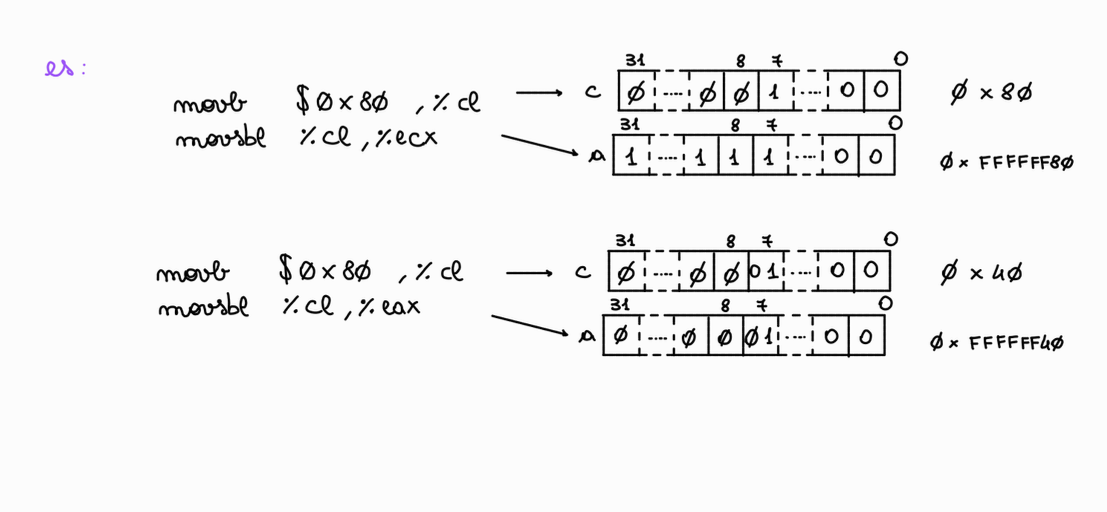
\includegraphics[width=0.9\linewidth]{../images/esempio char int.png}
        \caption{Esempio}
    \end{figure}
\end{enumerate}
\textit{Esempio}: \\
\begin{minipage}{0.4\textwidth}
    \begin{verbatim}
int f(char *p, char *q){
    int x = *p + *q;
    return x
}




    f.c
    \end{verbatim}
\end{minipage}
\hfill
$\longrightarrow$
\hfill
\begin{minipage}{0.4\textwidth}
    \begin{verbatim}
.globl f
f:
    movl 4(%esp), %eax  # A <-> p
    movl 8(%esp), %ecx  # C <-> q
    movsbl (%eax), %eax
    movsbl (%ecx), %ecx
    addl %ecx, %eax
    ret
    
    f.s
    \end{verbatim}
\end{minipage}\medskip\\
\textit{Altro esempio:} \medskip \\
\begin{minipage}{0.3\textwidth}
    \begin{verbatim}
int is_vowel(int c); 
// scritto nel mai e 
// restituisce 0/1
int num_vowels(char *s){
    int cnt = 0;
    while(*s)
        cnt += is_vowel(*s++);
    return cnt;
}

















    f.c
    \end{verbatim}
\end{minipage}
\hfill
$\longrightarrow$
\hfill
\begin{minipage}{0.2\textwidth}
    \begin{verbatim}
int is_vowel(int c);
int num_vowels(char *s){
    char *b = s;
    int di = 0 // di <-> cnt
L:
    if(*b == 0) goto E;
    int a = *b; 
    //ATTENZIONE: promozione
    a = is_vowel(a);
    di = di + a;
    b++;
    goto L;
E: 
    a = di;
    return a;
}










    f_eq.c
    \end{verbatim}
\end{minipage}
\hfill
$\longrightarrow$
\hfill
\begin{minipage}{0.2\textwidth}
    \begin{verbatim}
.globl num_vowels
num_vowels:
    #Prologo
    pushl %ebx
    pushl %edi
    subl $4(%esp)

    movl 16(%esp), %ebx
    xorl %edi, %edi
L:
    cmpb $0, (%ebx)
    je E
    movsbl %ebx, %eax
    movl %eax, (%esp)
    call is_vowel
    addl %eax, %edi
    incl %ebx
    jmp L
E:
    movl %edi, %eax
    #Epilogo
    addl $4(%esp)
    popl %edi
    popl %ebx
    ret
    
    f.s
    \end{verbatim}
\end{minipage}\medskip \\
\subsection{Variabili Locali}
Quando possibile, il compilatore utilizza i registri della CPU per memorizzare i valori delle variabili locali, poiché questa soluzione è la più semplice e garantisce le migliori prestazioni in termini di velocità di accesso. Tuttavia, non sempre ciò è possibile: in alcuni casi le variabili devono essere allocate nello \textit{stack frame} della funzione, cioè in memoria. Questo accade nei seguenti casi:
\begin{enumerate}
    \item \textbf{Registri insufficienti}: se il numero di variabili locali utilizzate dalla funzione supera quello dei registri disponibili, il compilatore è costretto a memorizzarne alcune nello stack.
    \item \textbf{Uso dell'operatore \&}: quando si applica l'operatore di indirizzo a una variabile locale, questa deve necessariamente risiedere in memoria, poiché deve avere un indirizzo ben definito.
    \item \textbf{Variabili complesse}: se la variabile è un array o una struttura (\texttt{struct}), non può essere contenuta interamente in un registro e quindi viene allocata nello stack.
\end{enumerate}
In sintesi, l'uso dei registri rappresenta un'ottimizzazione importante, ma è vincolato sia da limitazioni hardware (numero di registri) sia da requisiti semantici del programma (necessità di un indirizzo o dimensioni dei dati).
\begin{figure} [H]
    \centering
    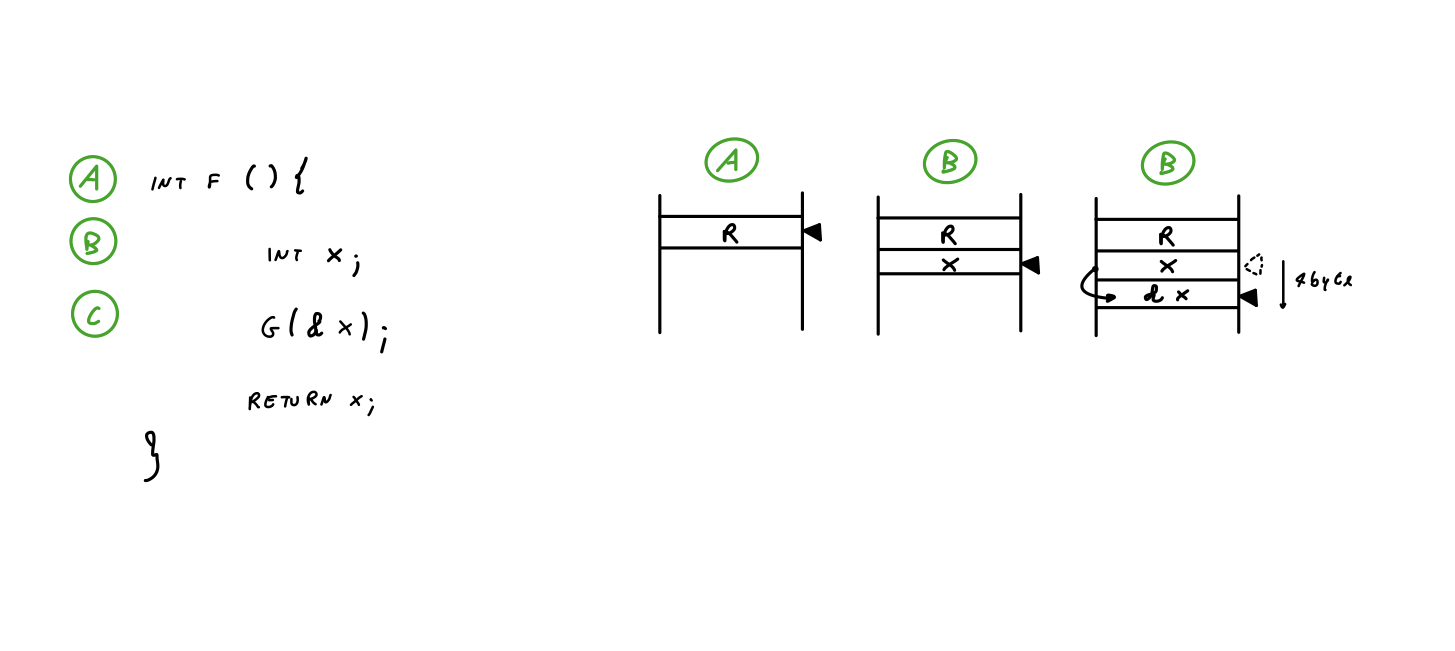
\includegraphics[width=1\linewidth]{../images/variabili locali.png}
    \caption{Caption}
    \label{fig:placeholder}
\end{figure}
\noindent Questo in assembly:
\begin{verbatim}
    .globl f
    f:
        #Prologo
        subl $8, %esp
        movl %esp, (%eax)   #lo salviamo in un registro
        addl $4, %eax       #poichè 'addl $4, (%esp)' non è corretto 
        #quindi per modificare il valore dovremmo prima portarlo in un altro registro
        movl %eax, (%esp)
        call g
        movl 4(%esp), %eax
        #Epilogo
        addl $8, %esp
        ret
\end{verbatim}
Nel dettaglio, la seguente sequenza di istruzioni:

\begin{verbatim}
movl %esp, (%eax)
addl $4, %eax  
\end{verbatim}
\noindent può essere riscritta in modo più compatto utilizzando l'istruzione \texttt{leal}:
\begin{verbatim}
leal 4(%esp), %eax
\end{verbatim}
\noindent L'istruzione \texttt{LEA} (Load Effective Address) consente di calcolare un indirizzo di memoria senza accedere effettivamente al contenuto di quella locazione. Si limita quindi a eseguire un calcolo aritmetico e a salvare il risultato in un registro. La sua forma generale è:
\begin{verbatim}
LEA O(B,I,S), D
\end{verbatim}
\noindent dove l'indirizzo calcolato è:

\[
B + I \cdot S + O
\]

\noindent In altre parole, il registro di destinazione viene aggiornato come segue:
\begin{itemize}
    \item inizialmente assume il valore base \(B\)
    \item viene aggiunto l'offset \(O\)
    \item viene aggiunto il contributo dell'indice \(I \cdot S\)
\end{itemize}

\noindent Per chiarire la differenza rispetto a \texttt{mov}, consideriamo il seguente confronto:

\medskip

\begin{minipage}{0.45\textwidth}
\begin{verbatim}
leal 4(%esp), %eax

calcola ESP + 4 e
scrive il risultato in EAX
\end{verbatim}
\end{minipage}
\hfill
$\longrightarrow$
\hfill
\begin{minipage}{0.45\textwidth}
\begin{verbatim}
movl 4(%esp), %eax

calcola ESP + 4, accede alla memoria
in quell'indirizzo e copia il valore
in EAX
\end{verbatim}
\end{minipage}

\medskip
\noindent Quindi, mentre \texttt{LEA} esegue solo un calcolo di indirizzi, \texttt{MOV} comporta anche un accesso alla memoria.\\
\textbf{\textcolor{red}{Importante}}: Se usiamo LEA per calcoli aritmetici lo status register (EFLAGS) NON viene alterato. Quindi non è da usare per le jump condizionate. \medskip \\
\begin{minipage}{0.3\textwidth}
    \begin{verbatim}
void get_div_rem(int *d,int *r, int x, int y);

inf f(int x, int y){
    int d, r;
    get_div_rem(&d,&r,x,y);
    return d;
}



    f.c
    \end{verbatim}
\end{minipage}
\hfill
$\longrightarrow$
\hfill
\begin{minipage}{0.4\textwidth}
    \begin{verbatim}
.globl f
f:
    #Prologo
    subl $24, %esp
    
    movl 28(%esp), %eax #x
    movl 32(%esp), %ecx #y

    leal 16(%esp),%edx  #&d
    movl %edx, (%esp)
    
    #stessa cosa per il secondo parametro
    leal 20(%esp), %edx #&r
    movl %edx,4(%esp)

    movl %eax, 8(%esp)
    movl %ecx, 12(%esp)

    call get_div_rem
    
    movl 16(%esp), %eax
    
    #Epilogo
    addl $24, %esp
    ret
    
    f.s
    \end{verbatim}
\end{minipage}\medskip \\
\begin{figure}[H]
    \centering
    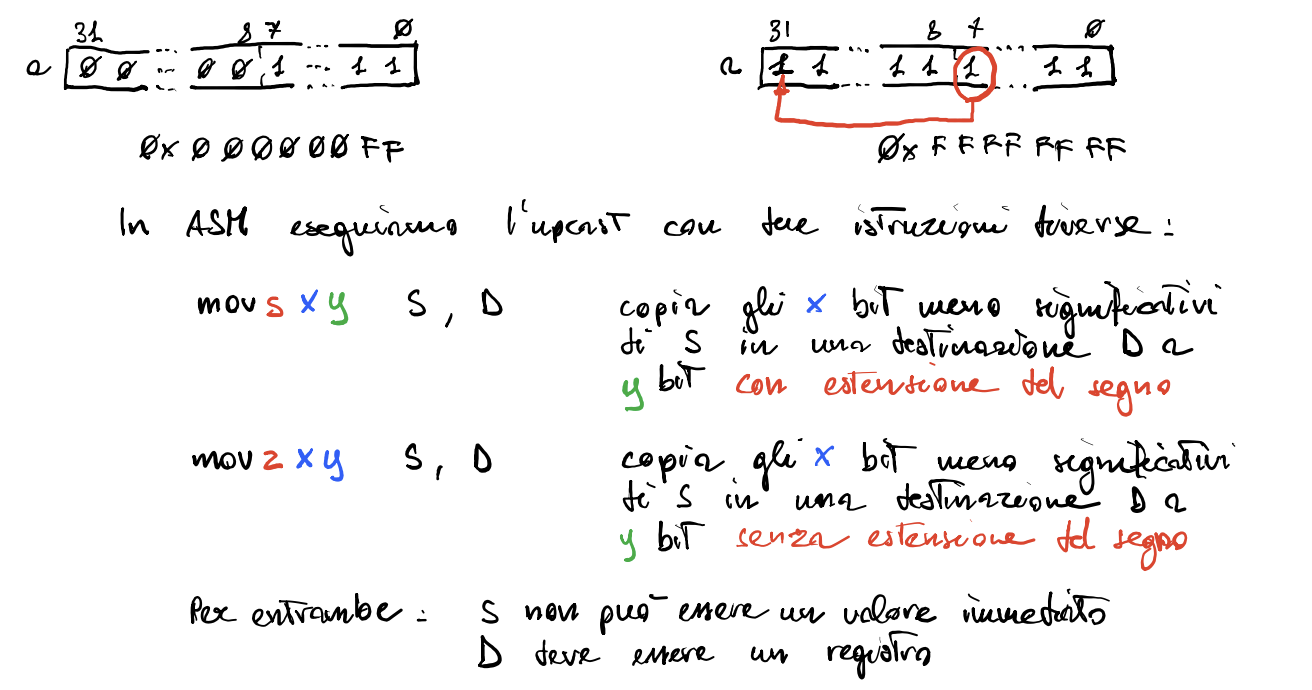
\includegraphics[width=0.9\linewidth]{../images/Esempio Movz xy.png}
    \caption{Graficamente}
    \label{label}
\end{figure}
\subsection{Espressioni Booleane}
L'istruzione \texttt{SETcc} (dove \texttt{cc} sta per \textit{condition code}) consente di assegnare il valore 0 oppure 1 a un registro a 8 bit oppure a un byte in memoria, in base al risultato di una condizione valutata sui flag contenuti nel registro \texttt{EFLAGS}. La forma generale dell'istruzione è:
\begin{verbatim}
SETcc D
\end{verbatim}
\noindent Il suo comportamento può essere descritto come:
\[
D \leftarrow \text{condizione}
\]
In particolare:
\begin{itemize}
    \item se la condizione associata al suffisso \texttt{cc} è verificata, viene scritto il valore 1 in \texttt{D1};
    \item altrimenti, viene scritto il valore 0.
\end{itemize}
Questa istruzione è spesso utilizzata per trasformare il risultato di un confronto in un valore booleano (0 o 1), utile ad esempio nelle espressioni condizionali. \medskip\\
\begin{minipage}{0.3\textwidth}
    \begin{verbatim}
int f(int x,int y){
    return x<y;
}
    \end{verbatim}
\end{minipage}
\hfill
$\longrightarrow$
\hfill
\begin{minipage}{0.3\textwidth}
    \begin{verbatim}
int f(int x,int y){
    int a = 1;
    if(x<y) goto E;
    a = 0;
    E:
        return a;
}
    \end{verbatim}
\end{minipage}
\hfill
$\longrightarrow$
\hfill
\begin{minipage}{0.3\textwidth}
    \begin{verbatim}
.globl f
f:
    movl 4(%esp), %eax  #x
    movl 8(%esp), %edx  #y
    cmpl %edx, %ecx
    setl %al    #restituisce un int
    movzbl %al, %eax
    ret
    \end{verbatim} 
\end{minipage}\medskip\\
\noindent Altro esempio: \medskip\\
\begin{minipage}{0.4\textwidth}
    \begin{verbatim}
int between(short x,short y, short z){
    return x<=y && y<=z;
}

f.c
    \end{verbatim}
\end{minipage}
\hfill
$\longrightarrow$
\hfill
\begin{minipage}{0.4\textwidth}
    \begin{verbatim}
.globl between
between:
    #Prologo
    pushl %ebx

    movw 8(%esp), %bx   #x
    movw 12(%esp), %cx  #y
    movw 16(%esp), %dx  #z

    cmpw %cx, %bx
    setle %al
    cmpw %dx, %cx
    stele %ah

    andb %ah, %al
    movzbl %al, %eax
    #Epilogo
    popl %ebx
    ret

f.s
    \end{verbatim}
\end{minipage}\medskip\\
\textbf{Regola del cortocircuito: differenza tra \texttt{\&} e \texttt{\&\&} in C}\\
In C esistono due operatori che possono sembrare simili ma hanno comportamenti diversi:
\begin{itemize}
    \item \texttt{\&\&} (AND logico): applica la \textbf{valutazione con cortocircuito}. La seconda espressione viene valutata \textbf{solo se} la prima è vera (diversa da zero). Se la prima è falsa, il risultato è già determinato e la seconda non viene eseguita.
    \item \texttt{\&} (AND bit a bit): \textbf{non utilizza il cortocircuito}. Entrambe le espressioni vengono sempre valutate, indipendentemente dal valore della prima.
\end{itemize}
In sintesi, il cortocircuito è una proprietà dell'operatore logico \texttt{\&\&}, mentre l'operatore \texttt{\&} esegue sempre entrambe le valutazioni.\\
\section{Allineamento nello Stack}

Consideriamo il seguente esempio:\medskip\\

\begin{minipage}{0.4\textwidth}
\begin{verbatim}
void g(char *c);

void f(){
    ...
    char a; // 1 byte
    g(&a);  // parametro: 4 byte
    ...
}
\end{verbatim}
\end{minipage}
\hfill
$\longrightarrow$
\hfill
\begin{minipage}{0.5\textwidth}
\begin{verbatim}
f:
    subl $4, %esp   # spazio per a (allineato a 4 byte)
    subl $4, %esp   # spazio per il parametro di g
    ...
    leal ...
    movl ..., (%esp)
    call g
    ...
\end{verbatim}
\end{minipage}

\medskip

\noindent\textbf{\textcolor{red}{Importante:}}  
In ogni momento dell'esecuzione, lo \texttt{stack pointer} deve essere allineato a un multiplo di 4 byte.  
In pratica, i compilatori moderni allineano lo stack a \textbf{16 byte}.
\begin{figure}[H]
    \centering  
    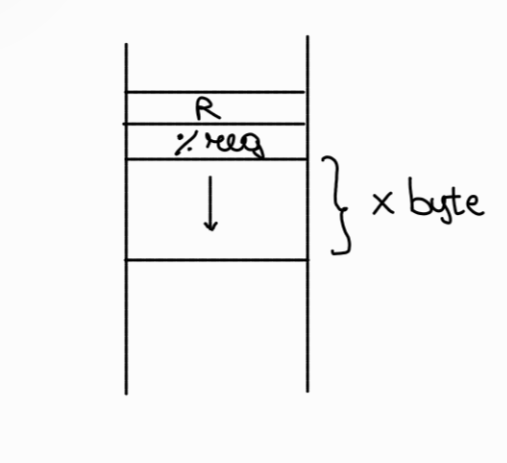
\includegraphics[width=0.3\linewidth]{../images/Allineamento in stack.png}
    \caption{SP}
    \label{label}
\end{figure}

\medskip

\noindent\textbf{Esempio con più variabili}: \medskip\\

\begin{minipage}{0.3\textwidth}
\begin{verbatim}
char a, b, c;
g(&a, &b, &c);
\end{verbatim}
\end{minipage}
\hfill
$\longrightarrow$
\hfill
\begin{minipage}{0.6\textwidth}
\begin{verbatim}
# Prologo
subl $16, %esp  # spazio totale

# Spiegazione:
# - a, b, c occupano 1 byte ciascuno
# - per allineamento diventano 4 byte ciascuno
# - parametri di g: 3 * 4 byte = 12 byte
# - totale: 3*4 + 12 = 24 → arrotondato a 16 (allineamento)
\end{verbatim}
\end{minipage}
\begin{figure}[H]
    \centering
    \includegraphics[width=0.3\linewidth]{../images/Esempio con più variabili.png}
    \caption{Ecco cosa succede nello SP}
    \label{label}
\end{figure}
\medskip
\noindent\textbf{\textcolor{red}{Regola fondamentale:}}  
Un dato di dimensione $x$ viene allocato a indirizzi multipli di $x$.

\medskip

\noindent\textbf{Altro esempio}:

\begin{minipage}{0.4\textwidth}
\begin{verbatim}
char a[5];
short b;
g(&a, &b);





f.c
\end{verbatim}
\end{minipage}
\hfill
$\longrightarrow$
\hfill
\begin{minipage}{0.5\textwidth}
\begin{verbatim}
# Prologo
subl $16, %esp

# Spiegazione:
# - a occupa 5 byte → allineato a 8 byte
# - b occupa 2 byte → allineato a 4 byte
# - parametri: 2 * 4 = 8 byte
# - totale: 8 + 4 + 8 = 20 → arrotondato a 16/32

f.s
\end{verbatim}
\end{minipage}

\bigskip

\section{Allineamento delle Struct}

Per tradurre una \texttt{struct} in Assembly, bisogna rispondere a:

\begin{enumerate}
    \item Dove inizia ogni campo in memoria?
    \item Quanto spazio occupa complessivamente la struct?
\end{enumerate}

\noindent\textbf{Regole di allineamento}:
\begin{enumerate}
    \item Un dato di dimensione $x$ deve essere allineato a indirizzi multipli di $x$
    \item L'allineamento della struct è determinato dal campo più grande
    \item La dimensione totale della struct è un multiplo della dimensione del campo più grande
\end{enumerate}
\textbf{Esempio (non ottimizzato)}

\begin{minipage}{0.4\textwidth}
\begin{verbatim}
struct s{
    char x;   // +0 |x - - -|
    int y;    // +4 |x x x x|
    short z;  // +8 |x x - -|
             // sizeof(s) = 12 (5 byte sprecati)
};

\end{verbatim}
\end{minipage}\bigskip\\
\noindent\textbf{Esempio (ottimizzato)}:\medskip\\
\begin{minipage}{0.4\textwidth}
\begin{verbatim}
struct s{
    char x;     // +0 |x -    
    short z;    // +2 |    x x|
    int y;      // +4 |x x x x|
                // sizeof(s) = 8 (1 byte sprecato)
};

\end{verbatim}
\end{minipage}

\medskip
\noindent\textbf{Nota:} Riordinare i campi riduce lo spazio sprecato e migliora l'efficienza.\\
\noindent\textbf{Esempio completo con Assembly}: \medskip\\
\begin{minipage}{0.4\textwidth}
\begin{verbatim}
struct s{
    char x; // +0
    int y;  // +4
};

void f(struct s *p, char a, int b){
    p->x = a;
    p->y = b;
}
\end{verbatim}
\end{minipage}
\hfill
$\longrightarrow$
\hfill
\begin{minipage}{0.4\textwidth}
\begin{verbatim}
.globl f
f:
    movl 4(%esp), %eax   # p
    movb 8(%esp), %cl    # a
    movl 12(%esp), %edx  # b

    movb %cl, (%eax)     # p->x
    movl %edx, 4(%eax)   # p->y

    ret
\end{verbatim}
\end{minipage}

\section{Allineamento Struct in memoria}
esempio:\medskip\\
\begin{minipage}{0.2\textwidth}
    \begin{verbatim} typedef struct nodo nodo;
    struct nodo{        base
        int elem;       +0 |xxxx|
        nodo *next;     +4 |xxxx|
    }                   sizeof nodo=8
    int sum(nodo *p){                   
        int count=0;                       
        for(;p;p=p->next)       
            count+=p->elem;               
        return count                        
    }            
    \end{verbatim}
\end{minipage}
\hfill
\hfill
$\longrightarrow$
\hfill
\begin{minipage}{0.2\textwidth}
    \begin{verbatim}
nodo *edx=p;
int eax=0;   //count
 L:  
 if(edx==NULL)
goto E;   
int ecx=edx->elem;
eax+=ecx;
edx=edx->next;
goto L;
E:
return eax;
}
    \end{verbatim}
\end{minipage}
\hfill
$\longrightarrow$
\hfill
\begin{minipage}{0.2\textwidth}
    \begin{verbatim}
.globl sum
sum:
    movl 4(%esp), %edx  
    xorl %eax, %eax  

L:
    testl %edx,%edx
    je E

    movl (%edx),%ecx
    addl %ecx,%eax
    movl 4(%edx),(%edx)
    jmp L
E:
    ret
    \end{verbatim} 
\end{minipage}\medskip\\
\noindent ESERCIZI SU 3.B-struct (vedi tu quale mettere tra questi che sono quelli fatti dal prof)\\
ESERCIZIO 1 SU PERSONA-ETA-GENDER\\
ESERCIZIO 2 SU FIND-YOUNGEST\\
\section{Istruzioni SHIFT}
\begin{verbatim}
                                ________________________________
    int a = ...;            a  |    .   |   .   |  .    |  .    |
    a = a >> 8;                 --------------------------------
                                        \       \       \       \___>scarto
                                ________________________________
                            a  |   ?    |   .   |  .    |   .   |
                                --------------------------------

                                ________________________________
    a = a << 8;             a  |    .   |   .   |   .   |   .   |  
                                --------------------------------
                  scartato <______/     /       /       /
                                ________________________________
                            a  |   .    |   .   |  .    |  ?    |  
                                --------------------------------
                                
\end{verbatim}  
\subsection{shift con segno}
\begin{verbatim}
    SAL S,D | D <- D << S   I nuovi bit meno significatavi sono posti uguali a 0
    SAR S,D | D <- D >> S   I nuovi bit più significativi sono posti uguali al
                            valore del bit più significativo
\end{verbatim}
\subsection{shift senza segno }
\begin{verbatim}
    SHL S,D | D <- D << S   I nuovi bit meno significatavi sono posti pari a 0
    SHR S,D | D <- D >> S   I nuovi bit meno significatavi sono posti pari a 0
\end{verbatim}
\noindent esepio:
\begin{verbatim}
    int c = 0xABADCAFE;
    unsigned d = 0xABADCAFE;
    c = c << 8;      // assembly: sall $8,%ecx       %ecx -> 0xADCAFE00
    d = d << 8;      // assembly: shll $8,%ecx       %ecx -> 0xADCAFE00
    c = c >> 8;      // assembly: sarl $8,%ecx       %ecx -> 0xFFADCAFE   
    d = d >> 8;      // assembly: shrl $8,%ecx       %ecx -> 0x00ADCAFE
\end{verbatim}
\noindent esempio:
\begin{verbatim}
    int  a = 8;      000....001000 -> 8
    a = a >> 2;      000....000010 -> 2 = 8/(2^2) esponente di 2 è il numero di bit shift
\end{verbatim}
\noindent $a >> x \rightarrow a/2^x$
\begin{verbatim}
    int  a = 8;      000....001000 -> 8
    a = a << 2;      000....100000 -> 32 = 8*(2^2) esponente di 2 è il numero di bit shift
\end{verbatim}
\noindent $a << x \rightarrow a \cdot 2^x$\medskip\\
esercizio:\medskip\\
\begin{minipage}{0.3\textwidth}
    \begin{verbatim}
unsigned count1(unsigned n){
    unsigned a=0;
    while(n>0){
        if(n & 1)a++;
        n = n >> 1;
    }
    return a;
}

e1.c
    \end{verbatim}
\end{minipage}
\hfill
$\longrightarrow$
\hfill
\begin{minipage}{0.3\textwidth}
    \begin{verbatim}
unsigned count1(unsigned n){
    unsigned eax=0;
    unsigned ecx=n;
L:
    if(c <= 0) goto E;
    if ((n & 1)==0) goto A;
    eax++;
A:
    ecx = ecx >> 1;
    goto L;
E:  
    return eax
}

e1_eq.c
    \end{verbatim}
\end{minipage}
\hfill
$\longrightarrow$
\hfill
\begin{minipage}{0.3\textwidth}
    \begin{verbatim}
.globl count1
count1:
    xorl %eax,%eax
    movl 4(%esp),%ecx
L:
    cmpl $0,%ecx
    jbe E
    testl $1,%ecx
    jz A
    incl %eax
A:
    shrl $1,%ecx
    jmp L
E:
    ret

e1.s
    \end{verbatim} 
\end{minipage}\medskip\\
\section{istruzione IDIV}
\begin{verbatim}
    idiv s  |   A <- D : A / S  quoziente
            |   D <- D : A % S  resto
\end{verbatim}
\noindent esempio:\\
\begin{minipage}{0.4\textwidth}
    \begin{verbatim}
int a = 20;
int c = 3;
a = a/c
    
f.c
    \end{verbatim}
\end{minipage}
\hfill
$\longrightarrow$
\hfill
\begin{minipage}{0.4\textwidth}
    \begin{verbatim}
movl $20,%eax              
movl $3,%ecx            

movl %eax,%edx      |   questa coppia di 
sarl $31,%edx       |   istruzioni prepara 
                    |   per i idiv

idiv %ecx

f.s
    \end{verbatim}
\end{minipage}\medskip\\
Esempio:\\
\begin{minipage}{0.3\textwidth}
    \begin{verbatim}
int f(int x, int y){
return x/y;
}

e1.c
    \end{verbatim}
\end{minipage}
\hfill
$\longrightarrow$
\hfill
\begin{minipage}{0.3\textwidth}
    \begin{verbatim}
int f(int x, int y){
    int a = x;
    int c = y;
    int d = a;
    d=d >> 31;
    a = a / c;
    return a;
}

e1_eq.c
    \end{verbatim}
\end{minipage}
\hfill
$\longrightarrow$
\hfill
\begin{minipage}{0.3\textwidth}
    \begin{verbatim}
.globl f
f:
    movl 4(%esp),%eax
    movl 8(%esp),%ecx
    movl %eax,%edx
    sarl $31,%edx
    idivl %ecx
    ret

e1.s
    \end{verbatim} 
\end{minipage}\medskip\\
\section{Istruzione CMOV}
\begin{verbatim}
    if (a>b) y=x;

    CMOVcc S,D  |   D <- S se cc è vero
                |   D <- D se cc è falso

    S non può essere un valore immediato
    D deve essere un registro a 16/32 bit
\end{verbatim}
\noindent Esempio\\
\begin{minipage}{0.3\textwidth}
    \begin{verbatim}
int max(int x, int y){
return (x > y) ? x : y;
}

e1.c
    \end{verbatim}
\end{minipage}
\hfill
$\longrightarrow$
\hfill
\begin{minipage}{0.3\textwidth}
    \begin{verbatim}
int max(int x, int y){
    int eax = x;
    int ecx = y;
    if(ecx > eax) 
        goto E;
    eax=ecx;
E:
    return eax;
    
}

e1_eq.c
    \end{verbatim}
\end{minipage}
\hfill
$\longrightarrow$
\hfill
\begin{minipage}{0.3\textwidth}
    \begin{verbatim}
.globl max
max:
    movl 4(%esp),%eax
    movl 8(%esp),%ecx
    cmpl %ecx,%eax
    cmovle %ecx,%eax  
    ret

e1.s
    \end{verbatim} 
\end{minipage}
\section{Ottimizzazione dei programmi}
Modificare un programma in modo che la sua esecuzione minimizzi l'uso delle risorse
disponibili, cercando allo stesso tempo di massimizzare le prestazioni, e senza 
alcun impatto sulla correttezza.\\
Problemi:\\
\begin{enumerate}
    \item Come posso valutare l'impatto che una modifica ha sul programma?\\
          Come misuro le prestazioni e l'uso delle risorse?
    \item Come posso scegliere le parti di un programma che voglio ottimizzare?\\
          Come identidico in un programma i "punti caldi" meritevoli di attenzione per possibili ottimizzazioni
\end{enumerate}
\noindent \subsection{Misure prestazionali}
\begin{itemize}
    \item \textbf{Latenza}: tempo necessario per eseguire il programma
    \item \textbf{Throughput}: numero di operazioni completate per unità di tempo
    \item \textbf{Spazio}: memoria utilizzata
    \item \textbf{Energia}
    \item \textbf{...}
\end{itemize}
\noindent \subsection{Analisi prestazionale del programma}
Quanto tempo richiede l'esecuzione di movl \$10,(\%eax) ? 
\begin{enumerate}
    \item Legge eax $\rightarrow$ $CPU + REG$       Maggiori prestazioni
    \item Scrive $10$ $\rightarrow$ Memoria RAM     Maggiori risorse       
\end{enumerate}
\noindent Il miglioramento prestazionale lo misuriamo come "speed up"\\
$speedup_o=\frac{t_o}{t'_0}$\\
otteniamo un numero adimensionale 2x\\
\textbf{Legge di Amdahl}\\
Ci permette di calcolare lo speedup complessivo di un programmaa fronte 
dell'ottimizzazione di una delle sue parti.\\
\begin{figure}
    \centering
    \includegraphics[width=0.5\linewidth]{../images/imagine}
    \caption{Caption}
    \label{fig:placeholder}
\end{figure}\\
$T = \alpha T + (1 - \alpha)T$\\
Ipotesi: posso ottimizzare A ottenendo per questo modulo uno speedup $k_A$\\
Qual'é lo speedup complessivo S di P?\\
$S=\frac{T}{T'} \quad T'=T'_A+T'_B=$\\
$=\frac{T_A}{k_A}+T_B=$\\
$=\frac{\alpha T}{k_A}+(1-\alpha)T=$\\
$=(\frac{\alpha}{k_A}+1-\alpha)T$\\
$S=\frac{T}{T'}=\frac{T}{(\frac{\alpha}{k_A}+1-\alpha)T}=\frac{1}{\frac{\alpha}{k_A}+1-\alpha}$\\
esempio: $\alpha=0,5 \quad k_A=2x \rightarrow s=1,33x$\\
esempio: $\alpha=0,9 \quad k_A=6x \rightarrow s=4x$\\
qual'è lo speedup teorico massimo?\\
$$\lim_{k_A\to\infty}\frac{1}{\frac{\alpha}{k_A}+1-\alpha}=\frac{1}{1-\alpha}$$

\newpage


\section{Istruzioni SHIFT}
Le istruzioni di shift (spostamento) in Assembly consentono di spostare 
i bit di un operando a sinistra o a destra. Esistono due tipi principali di shift:
\begin{itemize}
    \item \textbf{Shift con segno}
    \begin{verbatim}
        SAL S,D | D <- D << S   I nuovi bit meno significatavi sono posti uguali a 0
        SAR S,D | D <- D >> S   I nuovi bit più significativi sono posti uguali al
                                valore del bit più significativo
    \end{verbatim}
    \item \textbf{Shift senza segno}
    \begin{verbatim}
        SHL S,D | D <- D << S   I nuovi bit meno significatavi sono posti pari a 0
        SHR S,D | D <- D >> S   I nuovi bit meno significatavi sono posti pari a 0
    \end{verbatim}
\end{itemize}
\begin{figure}[H]
    \centering  
    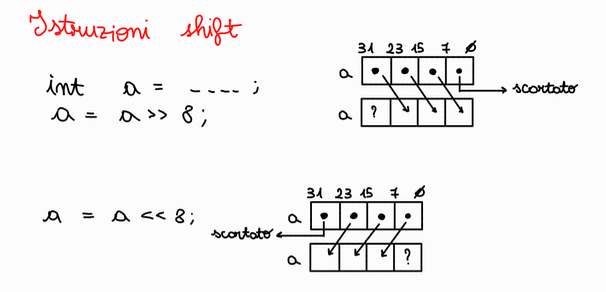
\includegraphics[width=0.8\linewidth]{../images/Shift.png}
    \caption{Shift dei bit}
    \label{label}
\end{figure}
\noindent Esempio:
\begin{verbatim}
    int c = 0xABADCAFE;
    unsigned d = 0xABADCAFE;
    c = c << 8;      // assembly: sall $8,%ecx       %ecx -> 0xADCAFE00
    d = d << 8;      // assembly: shll $8,%ecx       %ecx -> 0xADCAFE00
    c = c >> 8;      // assembly: sarl $8,%ecx       %ecx -> 0xFFADCAFE   
    d = d >> 8;      // assembly: shrl $8,%ecx       %ecx -> 0x00ADCAFE
\end{verbatim}
\noindent Esempio:
\begin{verbatim}
    int  a = 8;      000....001000 -> 8
    a = a >> 2;      000....000010 -> 2 = 8/(2^2) esponente di 2 è il numero di bit shift
\end{verbatim}
\noindent   $a >> x \rightarrow a/2^x$
\begin{verbatim}
    int  a = 8;      000....001000 -> 8
    a = a << 2;      000....100000 -> 32 = 8*(2^2) esponente di 2 è il numero di bit shift
\end{verbatim}
\noindent $a << x \rightarrow a \cdot 2^x$ \medskip\\
Vediamo ora attraverso un esercizio:\\
\begin{minipage}{0.3\textwidth}
    \begin{verbatim}
unsigned count1(unsigned n){
    unsigned a=0;
    while(n>0){
        if(n & 1)a++;
        n = n >> 1;
    }
    return a;
}







f.c
    \end{verbatim}
\end{minipage}
\hfill
$\longrightarrow$
\hfill
\begin{minipage}{0.3\textwidth}
    \begin{verbatim}
unsigned count1(unsigned n){
    unsigned eax=0;
    unsigned ecx=n;
L:
    if(c <= 0) goto E;
    if ((n & 1)==0) goto A;
    eax++;
A:
    ecx = ecx >> 1;
    goto L;
E:  
    return eax
}


f_eq.c
    \end{verbatim}
\end{minipage}
\hfill
$\longrightarrow$
\hfill
\begin{minipage}{0.3\textwidth}
    \begin{verbatim}
.globl count1
count1:
    xorl %eax,%eax
    movl 4(%esp),%ecx
L:
    cmpl $0,%ecx
    jbe E
    testl $1,%ecx
    jz A
    incl %eax
A:
    shrl $1,%ecx
    jmp L
E:
    ret

f.s
    \end{verbatim} 
\end{minipage}\medskip\\
\section{Istruzione IDIV}
\noindent L'istruzione \texttt{IDIV} esegue la divisione intera con segno 
tra il valore contenuto nel registro \texttt{EAX} (dividendo) e un operando 
specificato (divisore). Il risultato della divisione viene memorizzato in due registri:
\begin{itemize}
    \item Il quoziente (risultato della divisione) viene memorizzato in \texttt{EAX}.
    \item Il resto (modulo) viene memorizzato in \texttt{EDX}.
\end{itemize}
\begin{verbatim}
idiv s  |   A <- D : A / S  quoziente
        |   D <- D : A % S  resto
\end{verbatim}
Esempio:\\
\begin{minipage}{0.25\textwidth}
    \begin{verbatim}
int f(int x, int y){
return x/y;
}






f.c
    \end{verbatim}
\end{minipage}
\hfill
$\longrightarrow$
\hfill
\begin{minipage}{0.25\textwidth}
    \begin{verbatim}
int f(int x, int y){
    int a = x;
    int c = y;
    int d = a;
    d=d >> 31;
    a = a / c;
    return a;
}

f_eq.c
    \end{verbatim}
\end{minipage}
\hfill
$\longrightarrow$
\hfill
\begin{minipage}{0.4\textwidth}
    \begin{verbatim}
.globl f
f:
    movl 4(%esp),%eax
    movl 8(%esp),%ecx
    movl %eax,%edx      |   questa coppia di 
    sarl $31,%edx       |   istruzioni prepara 
    idivl %ecx          |   per i idiv
    ret

f.s
    \end{verbatim} 
\end{minipage}\medskip\\
\section{Istruzione CMOV}
L'istruzione \texttt{CMOVcc} (Conditional Move) consente di eseguire un'operazione 
di assegnamento condizionale, spostando il valore da una sorgente a una destinazione 
solo se una specifica condizione è soddisfatta. La forma generale dell'istruzione è:
\begin{verbatim}
CMOVcc S,D  |   D <- S se cc è vero
            |   D <- D se cc è falso

S non può essere un valore immediato
D deve essere un registro a 16/32 bit
\end{verbatim}
\noindent Esempio\\
\begin{minipage}{0.3\textwidth}
    \begin{verbatim}



int max(int x, int y){
return (x > y) ? x : y;
}





f.c
    \end{verbatim}
\end{minipage}
\hfill
$\longrightarrow$
\hfill
\begin{minipage}{0.3\textwidth}
    \begin{verbatim}
int max(int x, int y){
    int eax = x;
    int ecx = y;
    if(ecx > eax) 
        goto E;
    eax=ecx;
E:
    return eax;
    
}

f_eq.c
    \end{verbatim}
\end{minipage}
\hfill
$\longrightarrow$
\hfill
\begin{minipage}{0.3\textwidth}
    \begin{verbatim}


.globl max
max:
    movl 4(%esp),%eax
    movl 8(%esp),%ecx
    cmpl %ecx,%eax
    cmovle %ecx,%eax  
    ret



f.s
    \end{verbatim} 
\end{minipage}
\section{Ottimizzazione dei programmi}
L'ottimizzazione di un programma consiste nel modificarlo in modo da minimizzare 
l'uso delle risorse disponibili, cercando allo stesso tempo di massimizzare le prestazioni, 
senza compromettere la correttezza.\\
\noindent\textbf{Problemi principali}:
\begin{enumerate}
    \item Come valutare l'impatto di una modifica sul programma?\\
    In altre parole: come misurare le prestazioni e l'uso delle risorse?
    \item Come individuare le parti del programma da ottimizzare?\\
    Come identificare i \textit{punti caldi} (hot spots) che meritano attenzione?
\end{enumerate}
\noindent\textbf{Misure prestazionali}:
\begin{itemize}
    \item \textbf{Latenza}: tempo necessario per eseguire il programma
    \item \textbf{Throughput}: numero di operazioni completate per unità di tempo
    \item \textbf{Spazio}: memoria utilizzata
    \item \textbf{Energia}: consumo energetico
\end{itemize}
\subsection{Analisi prestazionale del programma}
Ad esempio, quanto tempo richiede l'esecuzione dell'istruzione:
\begin{center}
\texttt{movl \$10,(\%eax)} ?
\end{center}
Possiamo scomporre l'operazione in:
\begin{enumerate}
    \item Lettura del registro \texttt{eax} $\rightarrow$ CPU + registri (operazione veloce)
    \item Scrittura del valore $10$ in memoria $\rightarrow$ RAM (operazione più costosa)
\end{enumerate}
\noindent Il miglioramento prestazionale si misura tramite lo \textbf{speedup}:

\[
\text{speedup} = \frac{T}{T'}
\]

\noindent dove $T$ è il tempo di esecuzione originale e $T'$ quello ottimizzato.

\subsection{Legge di Amdahl}
La legge di Amdahl permette di calcolare lo speedup complessivo di un programma
quando si ottimizza solo una sua parte.\\
Sia:
\[
T = \alpha T + (1 - \alpha)T
\]
\noindent dove:
\begin{itemize}
    \item $\alpha$ è la frazione di tempo spesa nella parte ottimizzabile
    \item $(1 - \alpha)$ è la parte non ottimizzabile
\end{itemize}
\noindent Supponiamo di ottenere uno speedup $k_A$ sulla parte ottimizzabile. Allora:

\[
T' = \frac{\alpha T}{k_A} + (1 - \alpha)T
\]

\noindent Lo speedup complessivo diventa:

\[
S = \frac{T}{T'} = \frac{1}{\frac{\alpha}{k_A} + (1 - \alpha)}
\]

\noindent\textbf{Procedimento:}\smallskip\\
$S=\frac{T}{T'} \quad T'=T'_A+T'_B$
$= \frac{T_A}{k_A}+T_B$
$=\frac{\alpha T}{k_A}+(1-\alpha)T$
$=(\frac{\alpha}{k_A}+1-\alpha)T$\smallskip\\
$S=\frac{T}{T'}=\frac{T}{(\frac{\alpha}{k_A}+1-\alpha)T}=\frac{1}{\frac{\alpha}{k_A}+1-\alpha}$\\
\begin{figure}[H]
    \centering  
    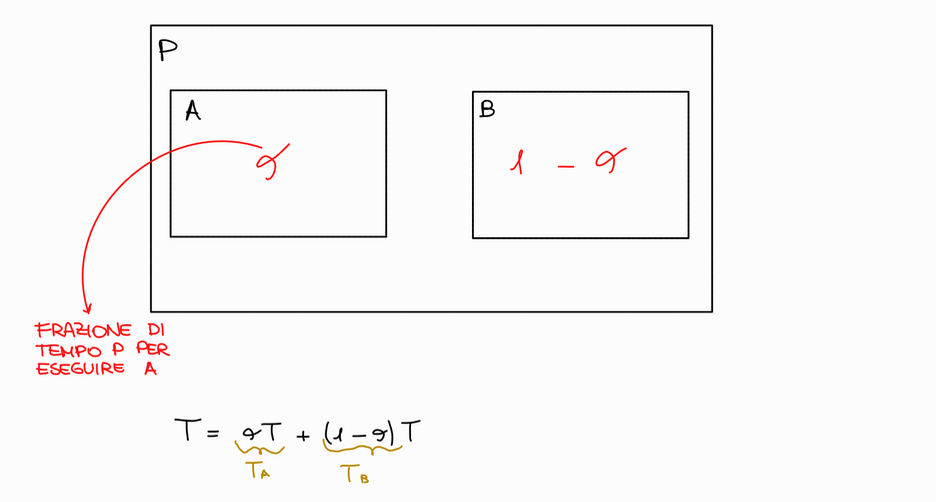
\includegraphics[width=0.7\linewidth]{../images/Legge di Amdahl.png}
    \caption{Legge di Amdahl}
\end{figure}

\noindent\textbf{Esempi}

\begin{itemize}
    \item $\alpha = 0.5$, $k_A = 2 \quad \Rightarrow \quad S \approx 1.33$
    \item $\alpha = 0.9$, $k_A = 6 \quad \Rightarrow \quad S \approx 4$
\end{itemize}

\noindent\textbf{Limite teorico}
\noindent Qual è lo speedup massimo ottenibile?

\[
\lim_{k_A \to \infty} \frac{1}{\frac{\alpha}{k_A} + (1 - \alpha)} 
= \frac{1}{1 - \alpha}
\]

\noindent Questo mostra che lo speedup è limitato dalla parte non ottimizzabile del programma.
